% !BIB TS-program = biber

\RequirePackage[l2tabu,orthodox]{nag}

% TODO: decide if one-sided/two-sided
%\documentclass[headsepline,footsepline,footinclude=false,fontsize=11pt,paper=a4,listof=totoc,bibliography=totoc,BCOR=12mm,DIV=12]{scrbook} % two-sided
\documentclass[headsepline,footsepline,footinclude=false,oneside,fontsize=10pt,paper=a4,listof=totoc,bibliography=totoc]{scrbook} % one-sided

% TODO: change citation style in settings
\PassOptionsToPackage{table,svgnames,dvipsnames}{xcolor}

\usepackage[utf8]{inputenc}
\usepackage[OT1]{fontenc}
\renewcommand*\familydefault{\sfdefault} %% Only if the base font of the document is to be sans serif
\usepackage[sc]{mathpazo}
\usepackage[ngerman,american]{babel}
\usepackage[autostyle]{csquotes}
\usepackage[%
  backend=biber,
  url=false,
  style=alphabetic,
  maxnames=4,
  minnames=3,
  maxbibnames=99,
  giveninits,
  uniquename=init]{biblatex} % TODO: adapt citation style
\usepackage{graphicx}
\usepackage{scrhack} % necessary for listings package
\usepackage{listings}
\usepackage{lstautogobble}
\usepackage{tikz}
\usepackage{pgfplots}
\usepackage{pgfplotstable}
\usepackage{booktabs}
\usepackage[final]{microtype}
\usepackage{caption}
\usepackage[printonlyused]{acronym}
\usepackage[hidelinks]{hyperref} % hidelinks removes colored boxes around references and links
\AtBeginDocument{%
	\hypersetup{
		pdftitle=\getTitle,
		pdfauthor=\getAuthor,
	}
}
\usepackage{ifthen}
\usepackage{geometry}
\geometry{hmargin=4.5cm, vmargin=4cm}

% for fachschaft_print.pdf
\makeatletter
\if@twoside
	\typeout{TUM-Dev LaTeX-Thesis-Template: twoside}
\else
	\typeout{TUM-Dev LaTeX-Thesis-Template: oneside}
\fi
\makeatother

\addto\extrasamerican{
	\def\lstnumberautorefname{Line}
	\def\chapterautorefname{Chapter}
	\def\sectionautorefname{Section}
	\def\subsectionautorefname{Subsection}
	\def\subsubsectionautorefname{Subsubsection}
}

\addto\extrasngerman{
	\def\lstnumberautorefname{Zeile}
}

% Themes
\ifthenelse{\equal{\detokenize{dark}}{\jobname}}{%
  % Dark theme
  \newcommand{\bg}{black} % background
  \newcommand{\fg}{white} % foreground
  \usepackage[pagecolor=\bg]{pagecolor}
  \color{\fg}
}{%
  % Light theme
  \newcommand{\bg}{white} % background
  \newcommand{\fg}{black} % foreground
}

\bibliography{bibliography}

\setkomafont{disposition}{\normalfont\bfseries} % use serif font for headings
\linespread{1.05} % adjust line spread for mathpazo font

% Add table of contents to PDF bookmarks
\BeforeTOCHead[toc]{{\cleardoublepage\pdfbookmark[0]{\contentsname}{toc}}}

% Define TUM corporate design colors
% Taken from http://portal.mytum.de/corporatedesign/index_print/vorlagen/index_farben
\definecolor{TUMBlue}{HTML}{0065BD}
\definecolor{TUMSecondaryBlue}{HTML}{005293}
\definecolor{TUMSecondaryBlue2}{HTML}{003359}
\definecolor{TUMBlack}{HTML}{000000}
\definecolor{TUMWhite}{HTML}{FFFFFF}
\definecolor{TUMDarkGray}{HTML}{333333}
\definecolor{TUMGray}{HTML}{808080}
\definecolor{TUMLightGray}{HTML}{CCCCC6}
\definecolor{TUMAccentGray}{HTML}{DAD7CB}
\definecolor{TUMAccentOrange}{HTML}{E37222}
\definecolor{TUMAccentGreen}{HTML}{A2AD00}
\definecolor{TUMAccentLightBlue}{HTML}{98C6EA}
\definecolor{TUMAccentBlue}{HTML}{64A0C8}

% Settings for pgfplots
\pgfplotsset{compat=newest}
\pgfplotsset{
  % For available color names, see http://www.latextemplates.com/svgnames-colors
  cycle list={TUMBlue\\TUMAccentOrange\\TUMAccentGreen\\TUMSecondaryBlue2\\TUMDarkGray\\},
}

% Settings for lstlistings
\lstset{%
  basicstyle=\ttfamily,
  columns=fullflexible,
  autogobble,
  keywordstyle=\bfseries\color{TUMBlue},
  stringstyle=\color{TUMAccentGreen},
  captionpos=b
}


% TODO: change thesis information
\newcommand*{\getUniversity}{École Polytechnique Fédérale de Lausanne}
\newcommand*{\getFaculty}{Computer Science}
\newcommand*{\getDegree}{Computer Science}
\newcommand*{\getSchool}{Computer and Communication Sciences}
\newcommand*{\getTitle}{Computer Vision Laboratory\\Unseen Spacecraft Pose Estimation}
\newcommand*{\getTitleGer}{Baseline solution implementation of a deep learning model for unseen spacecraft pose estimation}
\newcommand*{\getAuthor}{\textsc{Jérémy Chaverot}}
\newcommand*{\getDoctype}{Bachelor's Thesis}
\newcommand*{\getSupervisor}{Dr. \textsc{Mathieu Salzmann}}
\newcommand*{\getAdvisor}{Dr. \textsc{Andrew Price}, PhD. \textsc{Chen Zhao}}
\newcommand*{\getSemester}{Fall 2023}
\newcommand*{\getSubmissionDate}{26.01.24}
\newcommand*{\getSubmissionLocation}{Lausanne, Switzerland}

\begin{document}

% Set page numbering to avoid "destination with the same identifier has been already used" warning for cover page.
% (see https://en.wikibooks.org/wiki/LaTeX/Hyperlinks#Problems_with_Links_and_Pages).
\pagenumbering{alph}
\begin{titlepage}
  % HACK for two-sided documents: ignore binding correction for cover page.
  % Adapted from Markus Kohm's KOMA-Script titlepage=firstiscover handling.
  % See http://mirrors.ctan.org/macros/latex/contrib/koma-script/scrkernel-title.dtx,
  % \maketitle macro.
  \oddsidemargin=\evensidemargin\relax
  \textwidth=\dimexpr\paperwidth-2\evensidemargin-2in\relax
  \hsize=\textwidth\relax

  \centering

  \IfFileExists{logos/epfl-\fg.pdf}{%
    \includegraphics[height=20mm]{logos/epfl-\fg.pdf}
  }{%
    \vspace*{20mm}
  }

  \vspace{5mm}
  {\huge\MakeUppercase{School of \getSchool{}} \par}

  \vspace{5mm}
  {\large\MakeUppercase{\getUniversity{}} \par}

  \vspace{20mm}
  {\huge\bfseries \getTitle{} \par}
  
  \vspace{10mm}
  {\huge \foreignlanguage{ngerman}{\getTitleGer{}} \par}
  
  \vspace{15mm}
  {\Large \getDoctype{} in \getDegree{} \par}


  \vspace{15mm}
  \begin{tabular}{l l}
    Author:          & \getAuthor{}         \\
    Supervisor:      & \getSupervisor{}     \\
    Advisor:         & \getAdvisor{}        \\
    Submission Date: & \getSubmissionDate{} \\
  \end{tabular}

  \IfFileExists{logos/faculty-\fg.pdf}{%
    \vfill{}
    \includegraphics[height=20mm]{logos/faculty-\fg.pdf}
  }{}
\end{titlepage}


\frontmatter{}

%\addcontentsline{toc}{chapter}{Summary}
%\thispagestyle{empty}

%\vspace*{20mm}
\KOMAoptions{headsepline=false}

\begin{center}
    {\usekomafont{sectioning}\usekomafont{section}\textbf{\large Summary} }
\end{center}

This project falls within an Unseen 6 \ac{DoF} competition, organized in collaboration with the \ac{ESA} Advanced Concept Team. Essentially, we are dealing with space objects that are unfamiliar to us, and our objective is to accurately predict their 6\ac{DoF} poses. The action of the \ac{CVLab} team is twofold: firstly, we are tasked with creating a challenging dataset featuring multi-object, unseen, and occluded spacecraft scenarios. This involves ensuring a high degree of rendering realism. Secondly, we are focused on developing a baseline solution, which entails implementing a pose estimation model and conducting thorough training and testing on our dataset. My role this semester was primarily concentrated on the latter aspect, specifically on a track that incorporated target models.

\bigbreak 

Foremost, we started with a literature search by reading recent papers about generalizable 6DoF object pose estimation\footnote{\url{https://github.com/liuyuan-pal/Awesome-generalizable-6D-object-pose}}. Among the various models we explored, one that particularly captured our attention was the "Generalizable Model-Free 6-DoF Object Pose Estimation from RGB Images," commonly referred to as Gen6D \cite{liu2023gen6d}. We have compiled a table summarizing the advantages and disadvantages of this architecture for a clearer understanding:

\begin{table}[htpb]
  \caption[Example table]{Summary of Gen6D}\label{tab:sample}
  \centering
  \small
  \begin{tabular}{l | l}
    \toprule
      Pros & Cons \\
    \midrule
      Generalizability & Limited by Reference Image Quality \\
      Model-Free & Everyday Life Objects Training Data \\
      Simple Input Requirements & Difficulty with Symmetric Objects \\
      Robustness to Background Clutter & Dependence on Initial Detection and Selection \\
      Effective in Diverse Environments & Potential Challenges with Severe Occlusions \\
      Competitive Performance & Computationally Intensive \\
    \bottomrule
  \end{tabular}
\end{table}

We need to point out that Gen6D does not need a model because it uses a \ac{SFM} software called \textit{Colmap}. As we are on the track with the target models included, we simply skip this reconstruction step.

\bigbreak 

After selecting the model, we needed to establish a suitable environment for executing the code: EPFL Scitas Izar servers. Equipped with two NVIDIA V100 PCIe 32 GB GPUs, these servers are ideally configured for our \ac{ML} task. However, this stage proved to be more time-consuming than expected. It entailed various technical challenges, including setting up the virtual environment, installing the necessary dependencies, composing the bash execution script, and, fundamentally, learning the correct way to utilize the server.

After resolving the engineering aspects, we were able to delve into the practical side of the project, working directly with the code to adapt it to our dataset. After understanding the code, the initial task involved developing a data loader specifically for the Spacecraft dataset. This was accompanied by various minor modifications within the code, such as updating names and adjusting data paths. To align with the data format used by Gen6D for poses, it was necessary to write a Python script. This was because our dataset utilized quaternions combined with a translation vector in one text file, whereas Gen6D's format employed a rotation matrix augmented by the translation vector formatted as a separate numpy array for each image.

\KOMAoptions{headsepline=true}

Next, we tackled the debugging phase, aimed at addressing the model's accuracy issues. We encountered several problems. For instance, we needed to rectify the inverted masks for the objects using a Python script with the OpenCV library. Additionally, the model processes the reference images by cropping them into 128x128 pixel dimensions, while the detector is designed to identify objects in the query images that range from half to double the size of the reference images. Consequently, we resized the query images to reduce the scale difference relative to the reference images. This resizing was accompanied by necessary adjustments to the intrinsic matrix. Also we had to enhance the selection process of the reference images to ensure a more uniform distribution around the objects: contrary to everyday objects, spacecrafts can be observed from any angle, this should be considered in our approach.

\bigbreak 

One should bear in mind that in this model implementation, we decided to not retrain Gen6D. As a result, the outcomes are now more reliant than ever on the quality of the reference images. Given that we have access to highly realistic renderings of the spacecrafts and precise ground truth poses provided by the dataset team, we aim to assess Gen6D's effectiveness across a range of objects. Below are the visual results for the Hubble object:

\begin{figure}[h]
    \centering
    \begin{minipage}{0.45\linewidth}
        \centering
        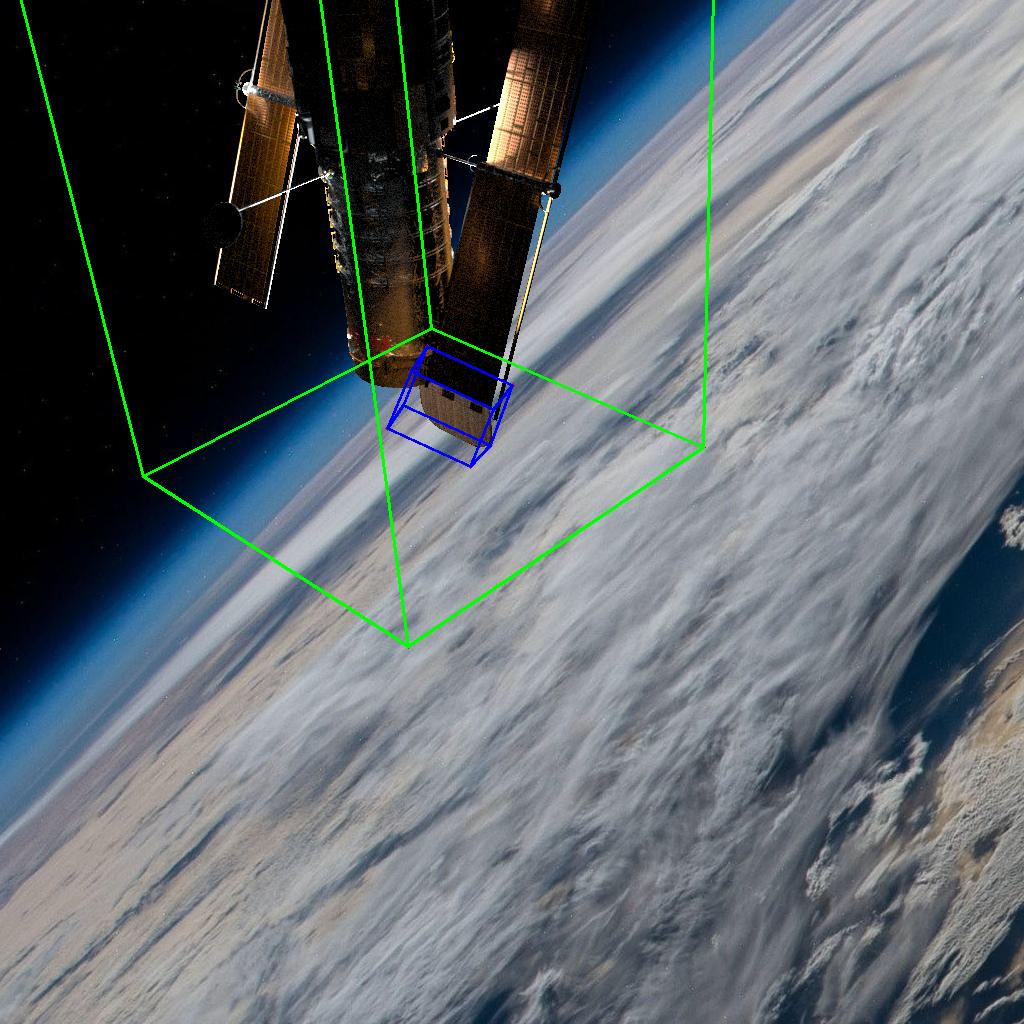
\includegraphics[width=\linewidth]{data/fig2.jpg} % First image
        \caption{Hubble Space Telescope with earth rendered background, 1024x1024 first query image}
        \label{fig:image1}
    \end{minipage}\hfill
    \begin{minipage}{0.45\linewidth}
        \centering
        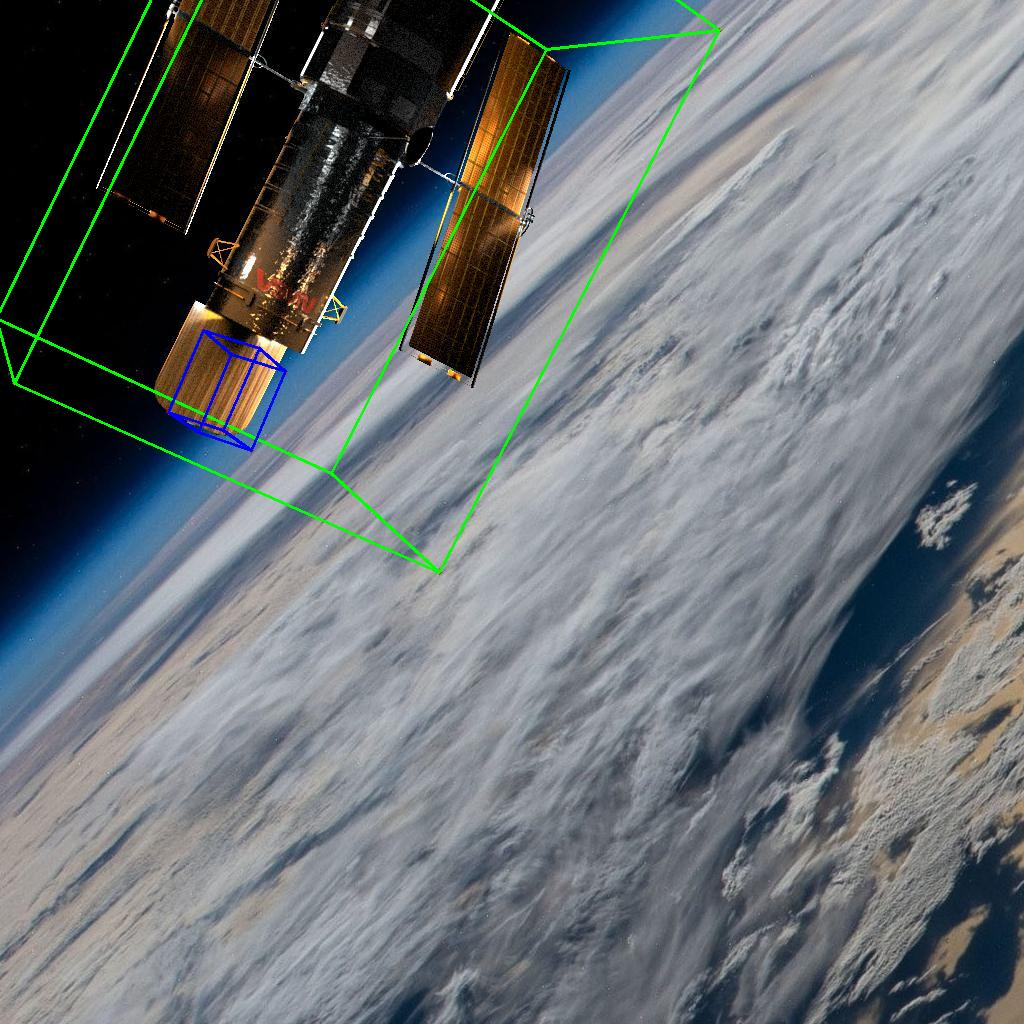
\includegraphics[width=\linewidth]{data/fig1.jpg} % Second image
        \caption{Hubble Space Telescope with earth rendered background, 1024x1024 second query image}
        \label{fig:image2}
    \end{minipage}
\end{figure}

\begin{figure}[h]
    \centering
    \begin{minipage}{0.45\linewidth}
        \centering
        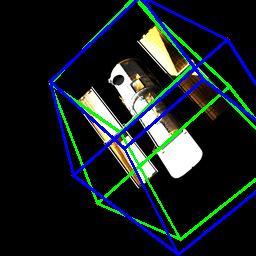
\includegraphics[width=\linewidth]{data/fig3.jpg} % First image
        \caption{Hubble Space Telescope, no background, 256x256 query image, $e_\mathrm{ADD}=2.925$, $e_{\mathrm{ADD}\text{-}\mathrm{S}}=1.183$ }
        \label{fig:image1}
    \end{minipage}\hfill
    \begin{minipage}{0.45\linewidth}
        \centering
        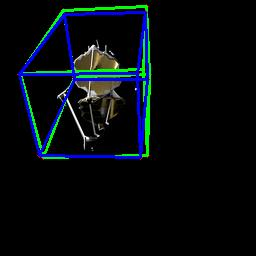
\includegraphics[width=\linewidth]{data/fig4.jpg} % Second image
        \caption{James Webb Space Telescope, no background, 256x256 query image, $e_\mathrm{ADD}=1.415$, $e_{\mathrm{ADD}\text{-}\mathrm{S}}=0.808$ }
        \label{fig:image2}
    \end{minipage}
\end{figure}

\begin{figure}[h]
    \centering
    \begin{minipage}{0.45\linewidth}
        \centering
        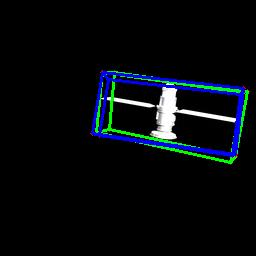
\includegraphics[width=\linewidth]{data/fig5.jpg} % First image
        \caption{Cosmos Link, no background, 256x256 query image, $e_\mathrm{ADD}=1.718$, $e_{\mathrm{ADD}\text{-}\mathrm{S}}=0.383$ }
        \label{fig:image1}
    \end{minipage}\hfill
    \begin{minipage}{0.45\linewidth}
        \centering
        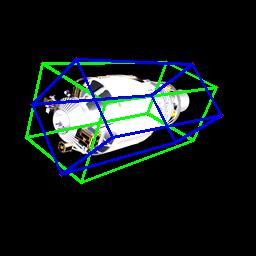
\includegraphics[width=\linewidth]{data/fig6.jpg} % Second image
        \caption{Rocket Body, no background, 256x256 query image, $e_\mathrm{ADD}=1.713$, $e_{\mathrm{ADD}\text{-}\mathrm{S}}=0.252$ }
        \label{fig:image2}
    \end{minipage}
\end{figure}

\begin{figure}[h]
    \centering
    \begin{minipage}{0.45\linewidth}
        \centering
        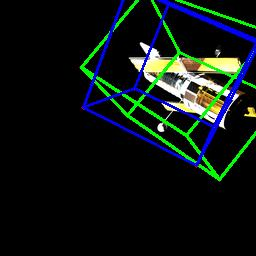
\includegraphics[width=\linewidth]{data/fig7.jpg} % First image
        \caption{Hubble Space Telescope, no background, 256x256 query image, $e_\mathrm{ADD}=6.514$, $e_{\mathrm{ADD}\text{-}\mathrm{S}}=1.571$ }
        \label{fig:image1}
    \end{minipage}\hfill
    \begin{minipage}{0.45\linewidth}
        \centering
        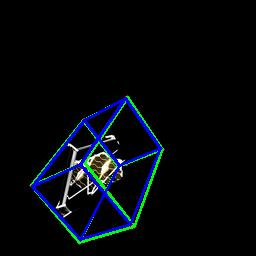
\includegraphics[width=\linewidth]{data/fig8.jpg} % Second image
        \caption{James Webb Space Telescope, no background, 256x256 query image, $e_\mathrm{ADD}=2.224$, $e_{\mathrm{ADD}\text{-}\mathrm{S}}=1.261$ }
        \label{fig:image2}
    \end{minipage}
\end{figure}

\begin{figure}[h]
    \centering
    \begin{minipage}{0.45\linewidth}
        \centering
        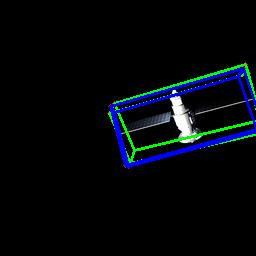
\includegraphics[width=\linewidth]{data/fig9.jpg} % First image
        \caption{Cosmos Link, no background, 256x256 query image, $e_\mathrm{ADD}=1.925$, $e_{\mathrm{ADD}\text{-}\mathrm{S}}=0.377$ }
        \label{fig:image1}
    \end{minipage}\hfill
    \begin{minipage}{0.45\linewidth}
        \centering
        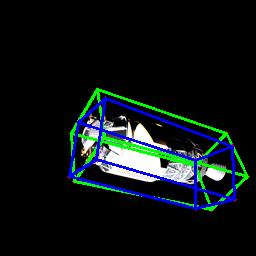
\includegraphics[width=\linewidth]{data/fig10.jpg} % Second image
        \caption{Rocket Body, no background, 256x256 query image, $e_\mathrm{ADD}=1.982$, $e_{\mathrm{ADD}\text{-}\mathrm{S}}=0.501$ }
        \label{fig:image2}
    \end{minipage}
\end{figure}

\begin{figure}[ht]
  \centering
  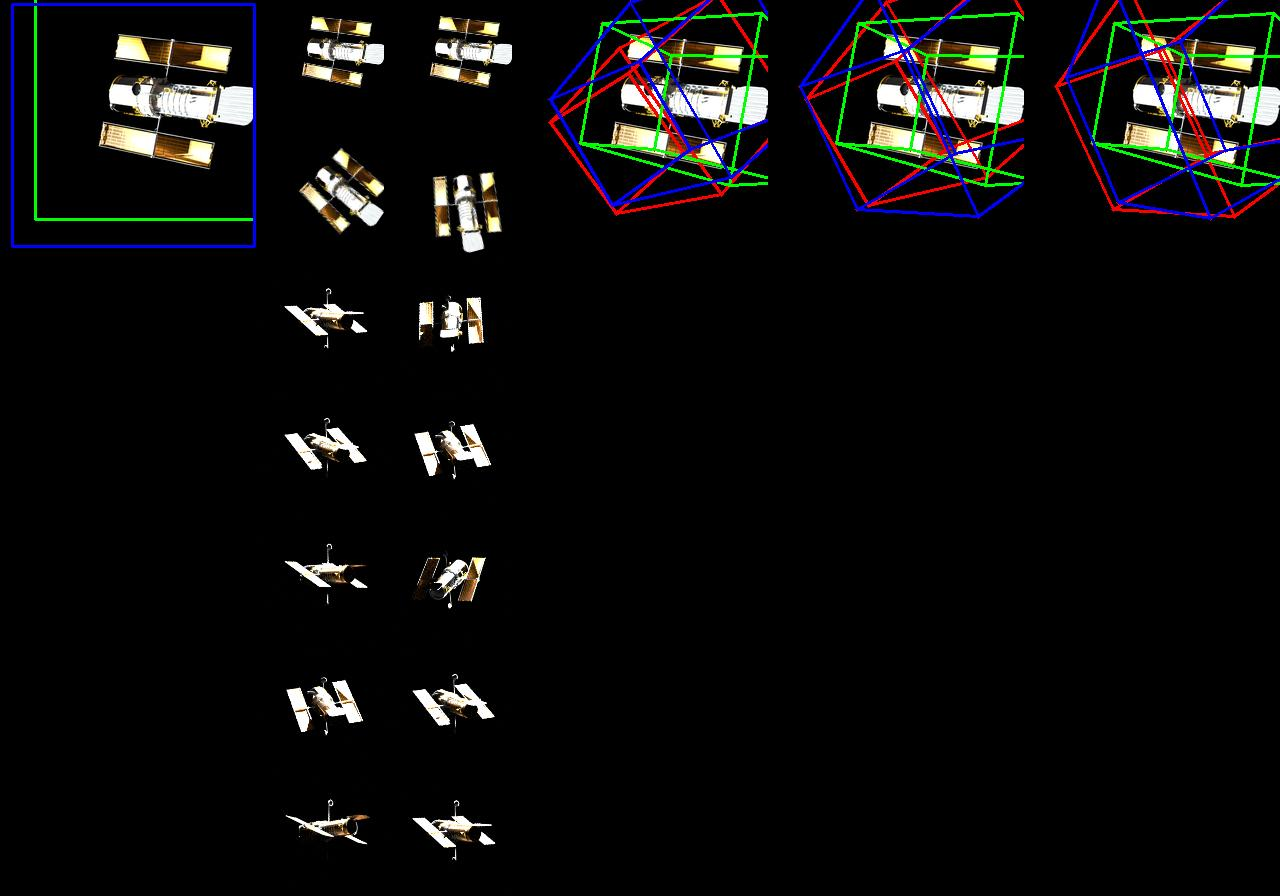
\includegraphics[width=\textwidth]{data/fig11.jpg}
  \caption{Hubble Space Telescope, no background, intermediary result, $e_\mathrm{ADD}=9.577$, $e_{\mathrm{ADD}\text{-}\mathrm{S}}=5.196$}
  \label{fig:cap1}
\end{figure}

\begin{figure}[ht]
  \centering
  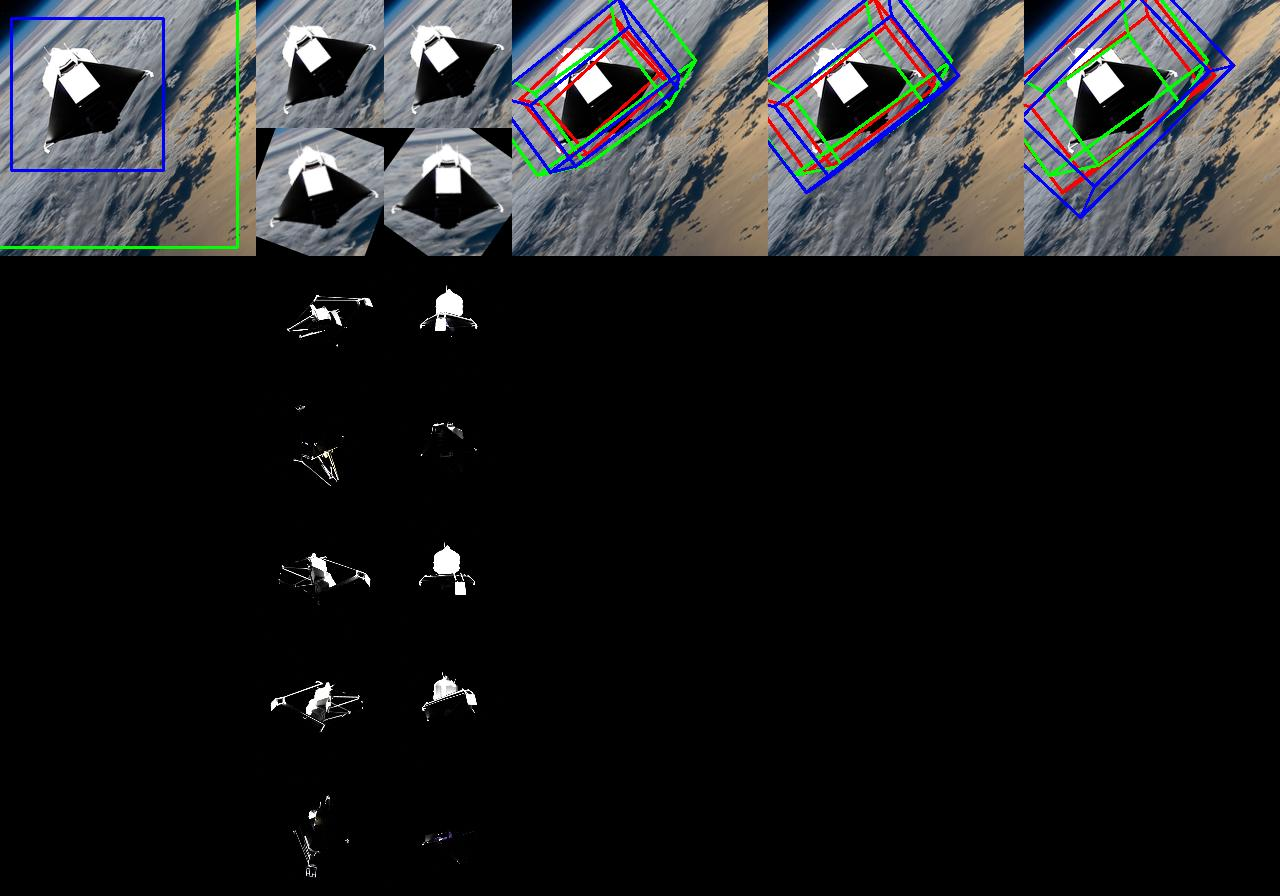
\includegraphics[width=\textwidth]{data/fig12.jpg}
  \caption{James Webb Space Telescope, with earth rendered background, intermediary result, $e_\mathrm{ADD}=10.934$, $e_{\mathrm{ADD}\text{-}\mathrm{S}}=4.317$}
  \label{fig:cap1}
\end{figure}

\begin{figure}[ht]
  \centering
  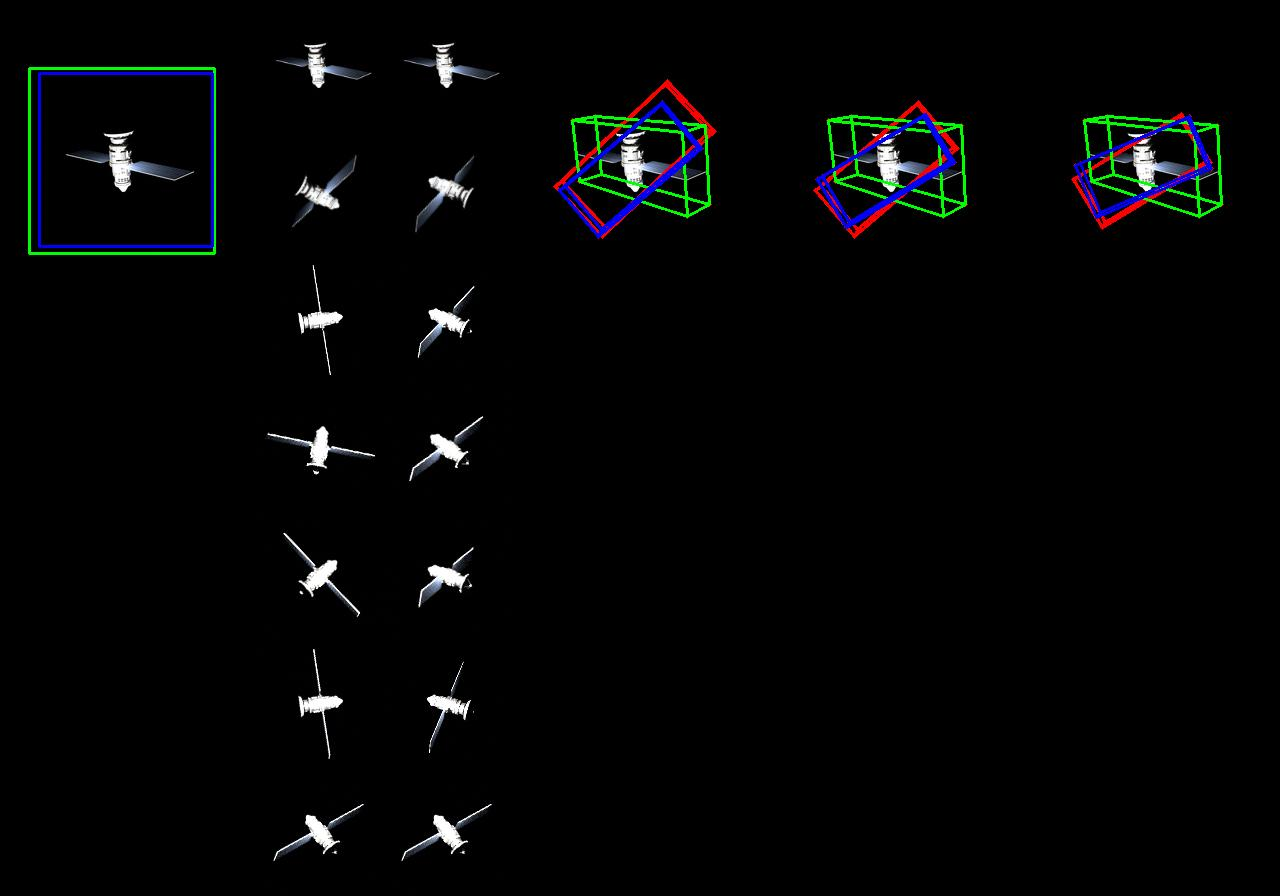
\includegraphics[width=\textwidth]{data/fig13.jpg}
  \caption{Cosmos Link, no background, intermediary result, $e_\mathrm{ADD}=11.094$, $e_{\mathrm{ADD}\text{-}\mathrm{S}}=6.127$}
  \label{fig:cap1}
\end{figure}

\begin{figure}[ht]
  \centering
  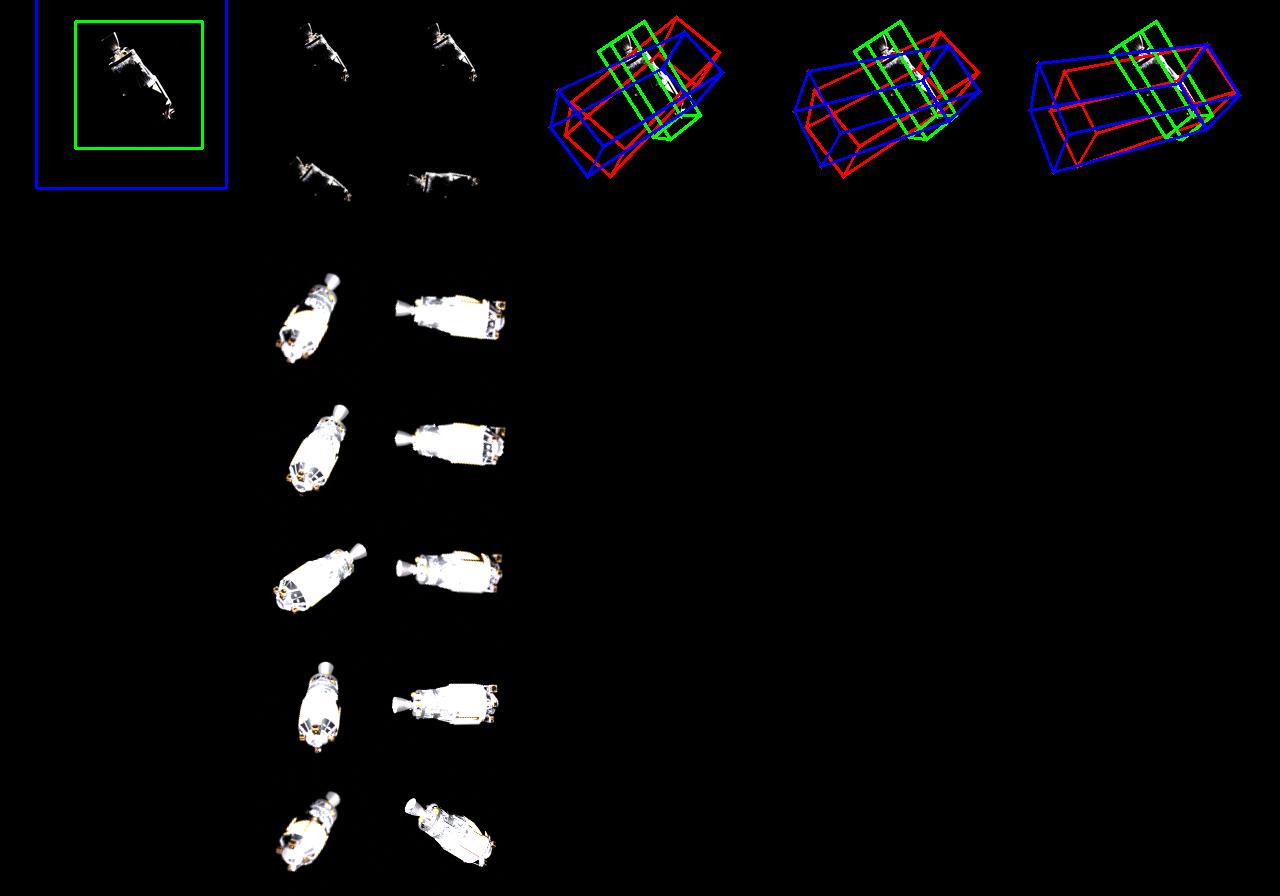
\includegraphics[width=\textwidth]{data/fig14.jpg}
  \caption{Rocket Body, no background, intermediary result, $e_\mathrm{ADD}=29.335$, $e_{\mathrm{ADD}\text{-}\mathrm{S}}=17.743$}
  \label{fig:cap1}
\end{figure}

\begin{figure}[ht]
  \centering
  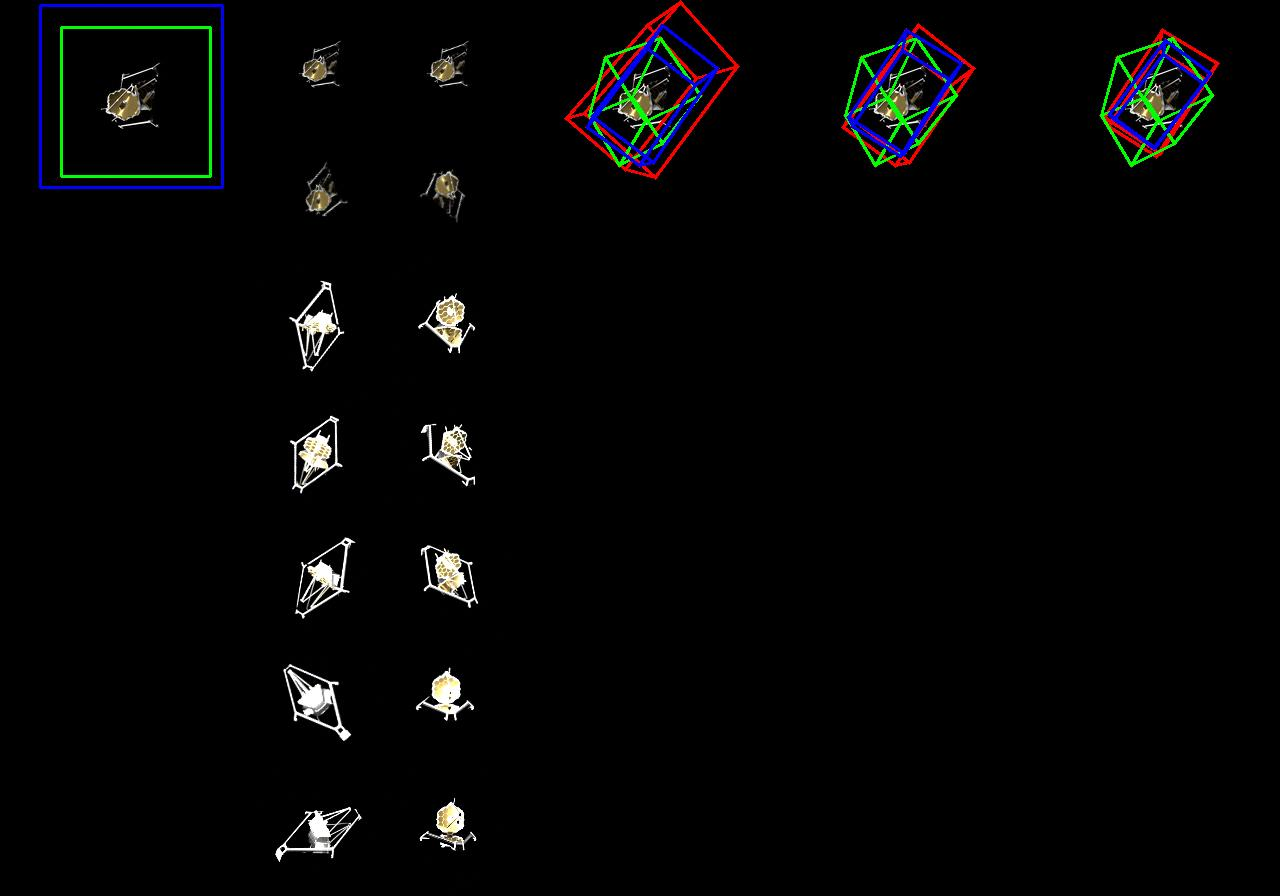
\includegraphics[width=\textwidth]{data/fig15.jpg}
  \caption{James Webb Space Telescope, with no background, intermediary result, $e_\mathrm{ADD}=21.983$, $e_{\mathrm{ADD}\text{-}\mathrm{S}}=12.358$}
  \label{fig:cap1}
\end{figure}

\begin{figure}[ht]
  \centering
  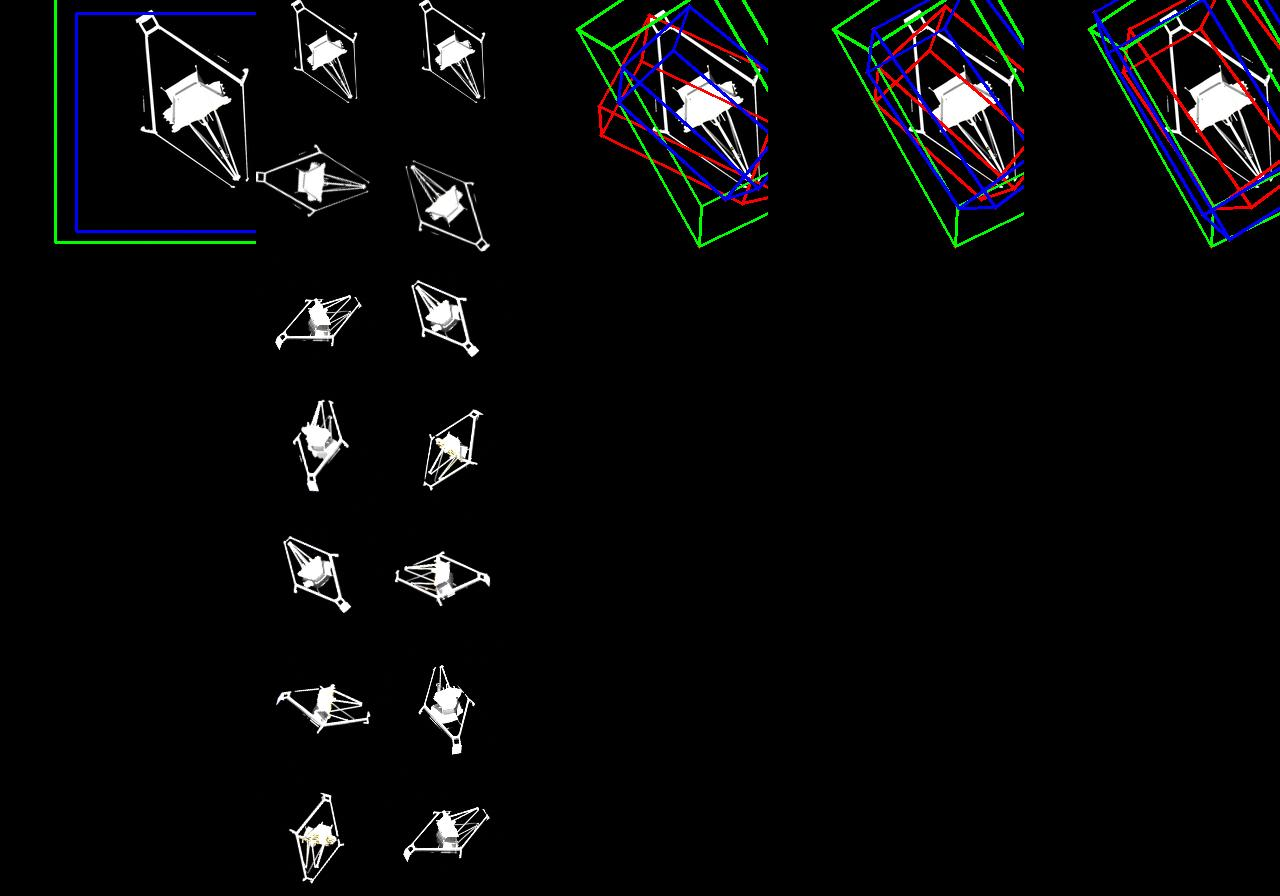
\includegraphics[width=\textwidth]{data/fig16.jpg}
  \caption{James Webb Space Telescope, with no background, intermediary result, $e_\mathrm{ADD}=1.060$, $e_{\mathrm{ADD}\text{-}\mathrm{S}}=0.556$}
  \label{fig:cap1}
\end{figure}

\begin{figure}[ht]
  \centering
  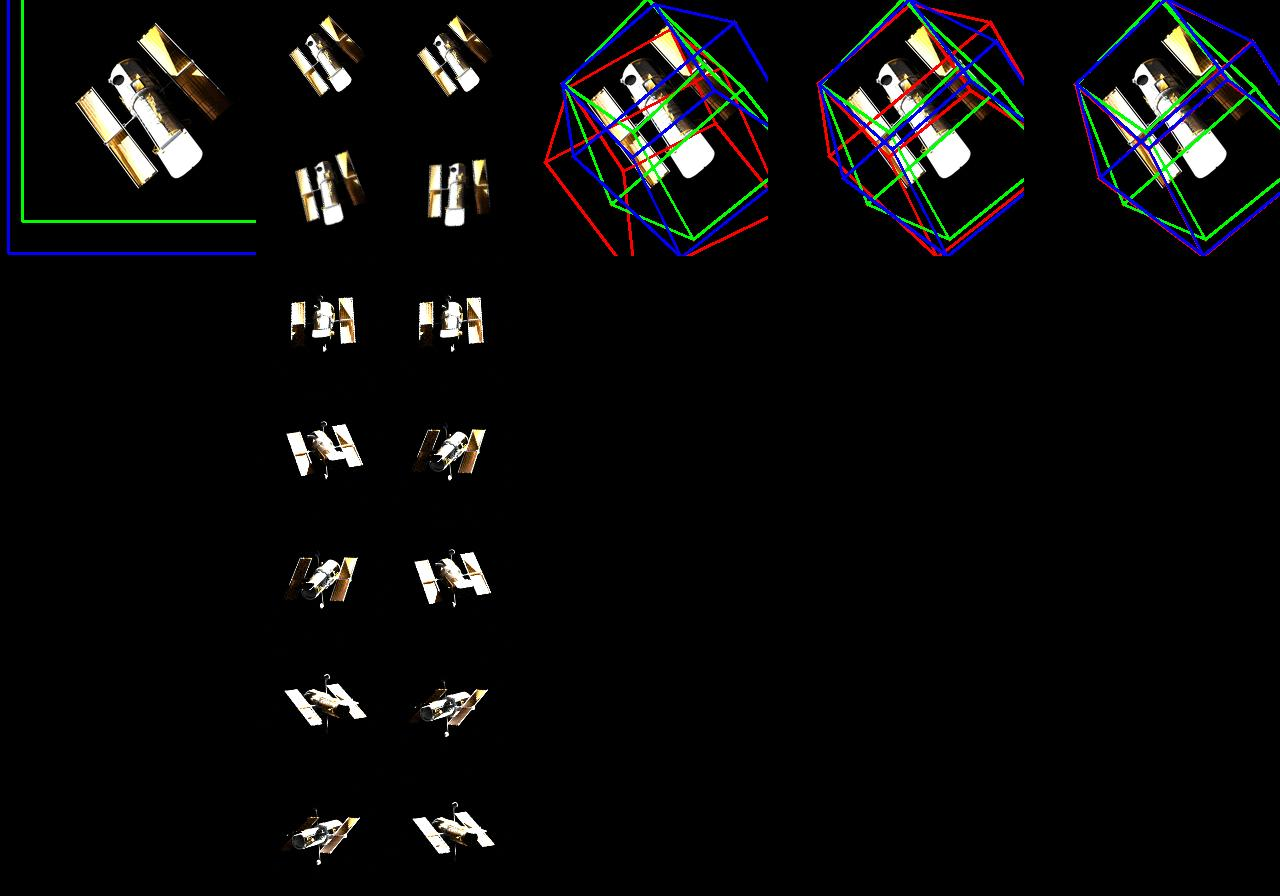
\includegraphics[width=\textwidth]{data/res2.jpg}
  \caption{An Estimation by Gen6D (Highlighted in Blue) of the Hubble Object, Presented Without a Background.} 
  \label{fig:cap1}
\end{figure}

\begin{figure}[ht]
  \centering
  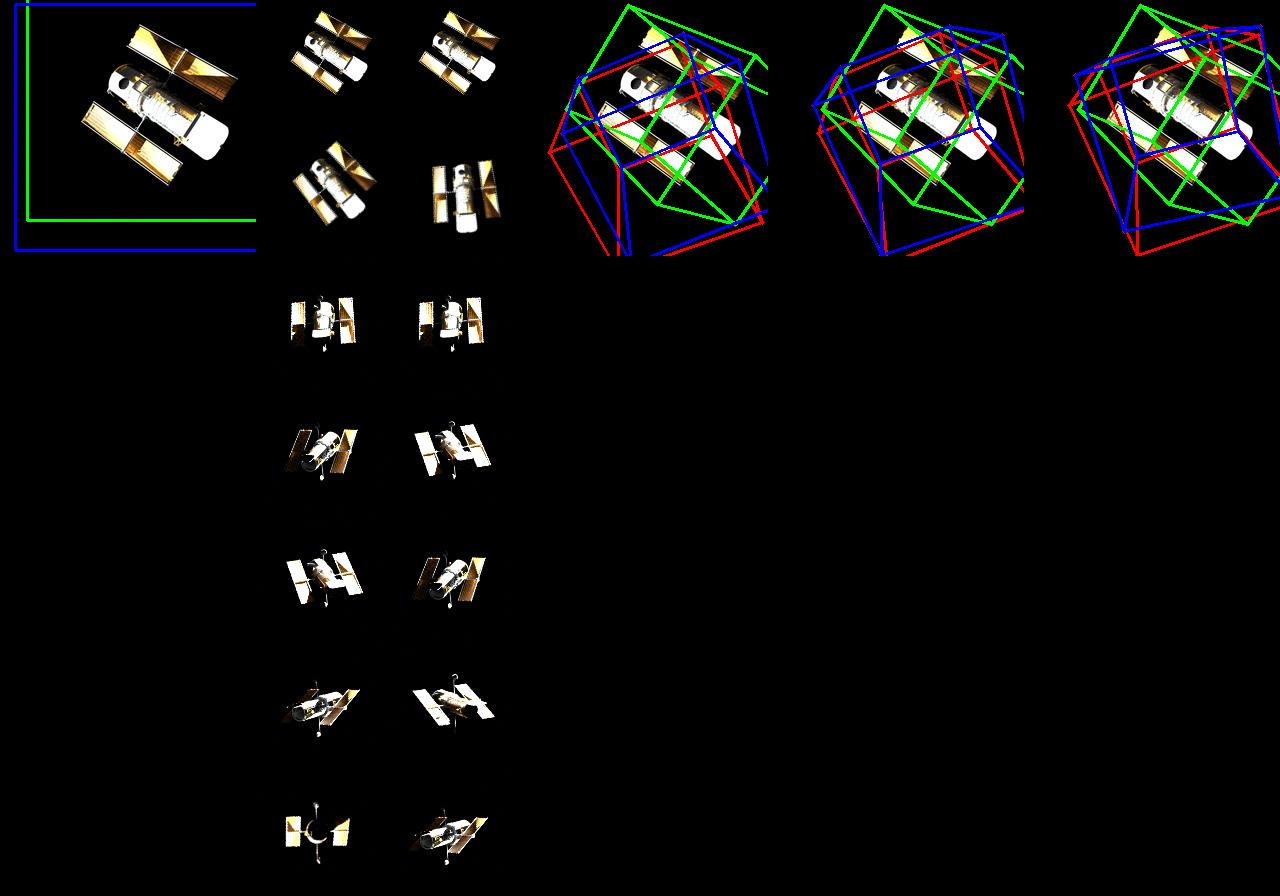
\includegraphics[width=\textwidth]{data/res3.jpg}
  \caption{An Estimation by Gen6D (Highlighted in Blue) of the Hubble Object, Presented Without a Background. Gen6D happens to lack of accuracy.}
  \label{fig:cap1}
\end{figure}

\begin{figure}[ht]
  \centering
  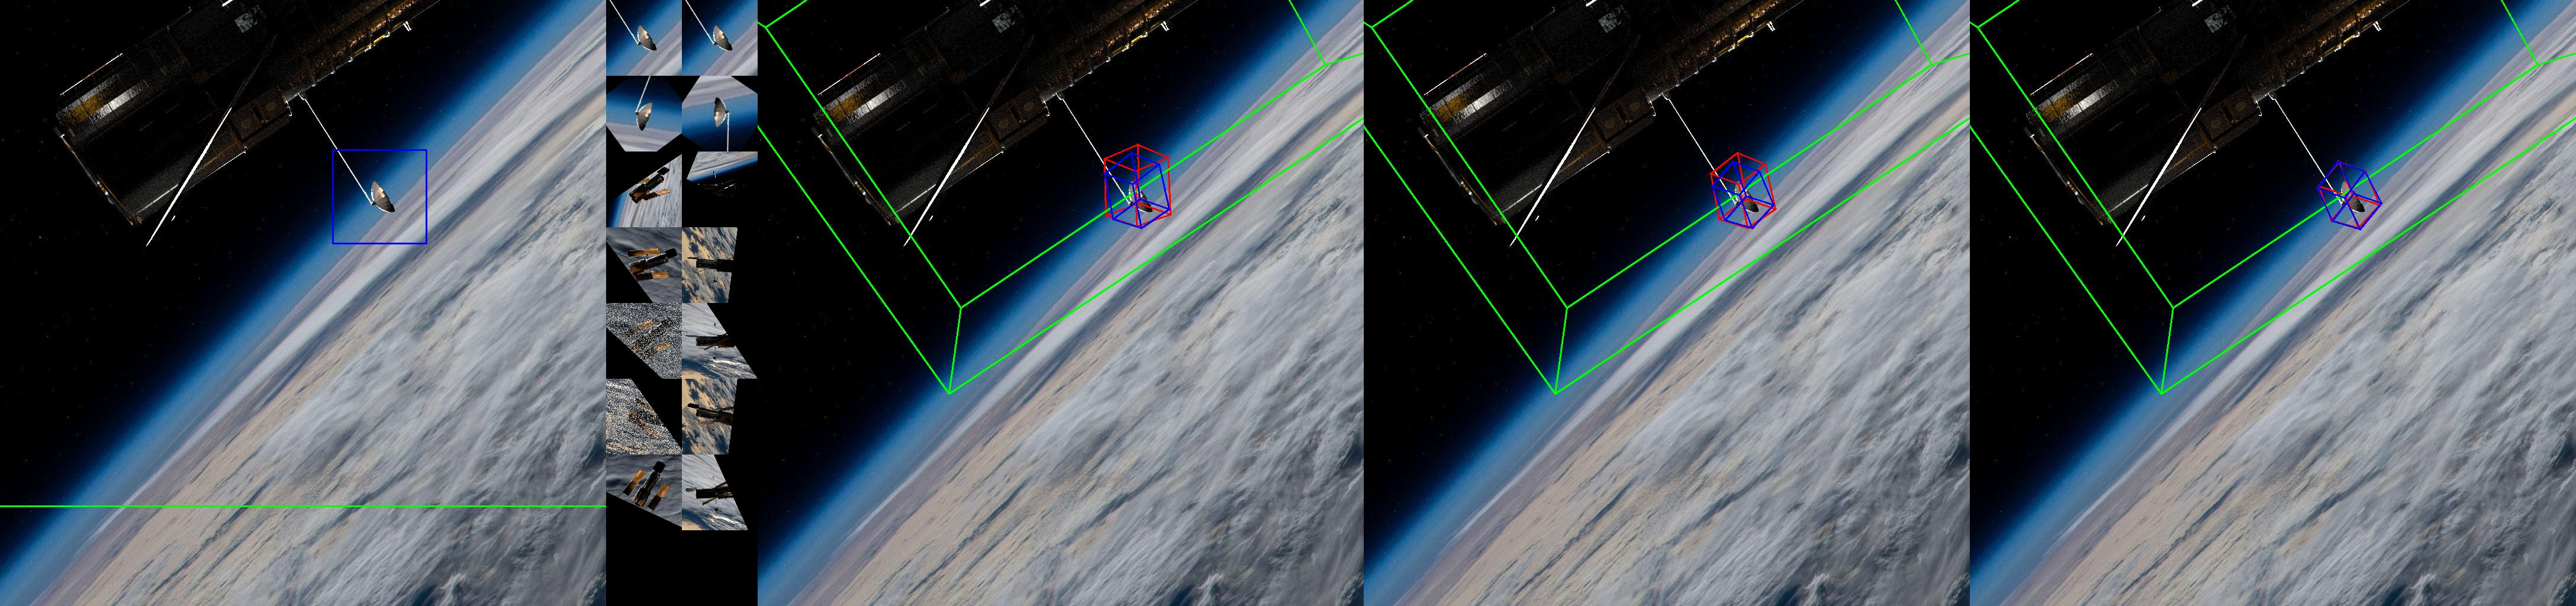
\includegraphics[width=\textwidth]{data/res4.jpg}
  \caption{An Estimation by Gen6D (Highlighted in Blue) of the Hubble Object, Presented With a Background. Here the query object size is too big for the detector.}
  \label{fig:cap4}
\end{figure}

\begin{figure}[ht]
  \centering
  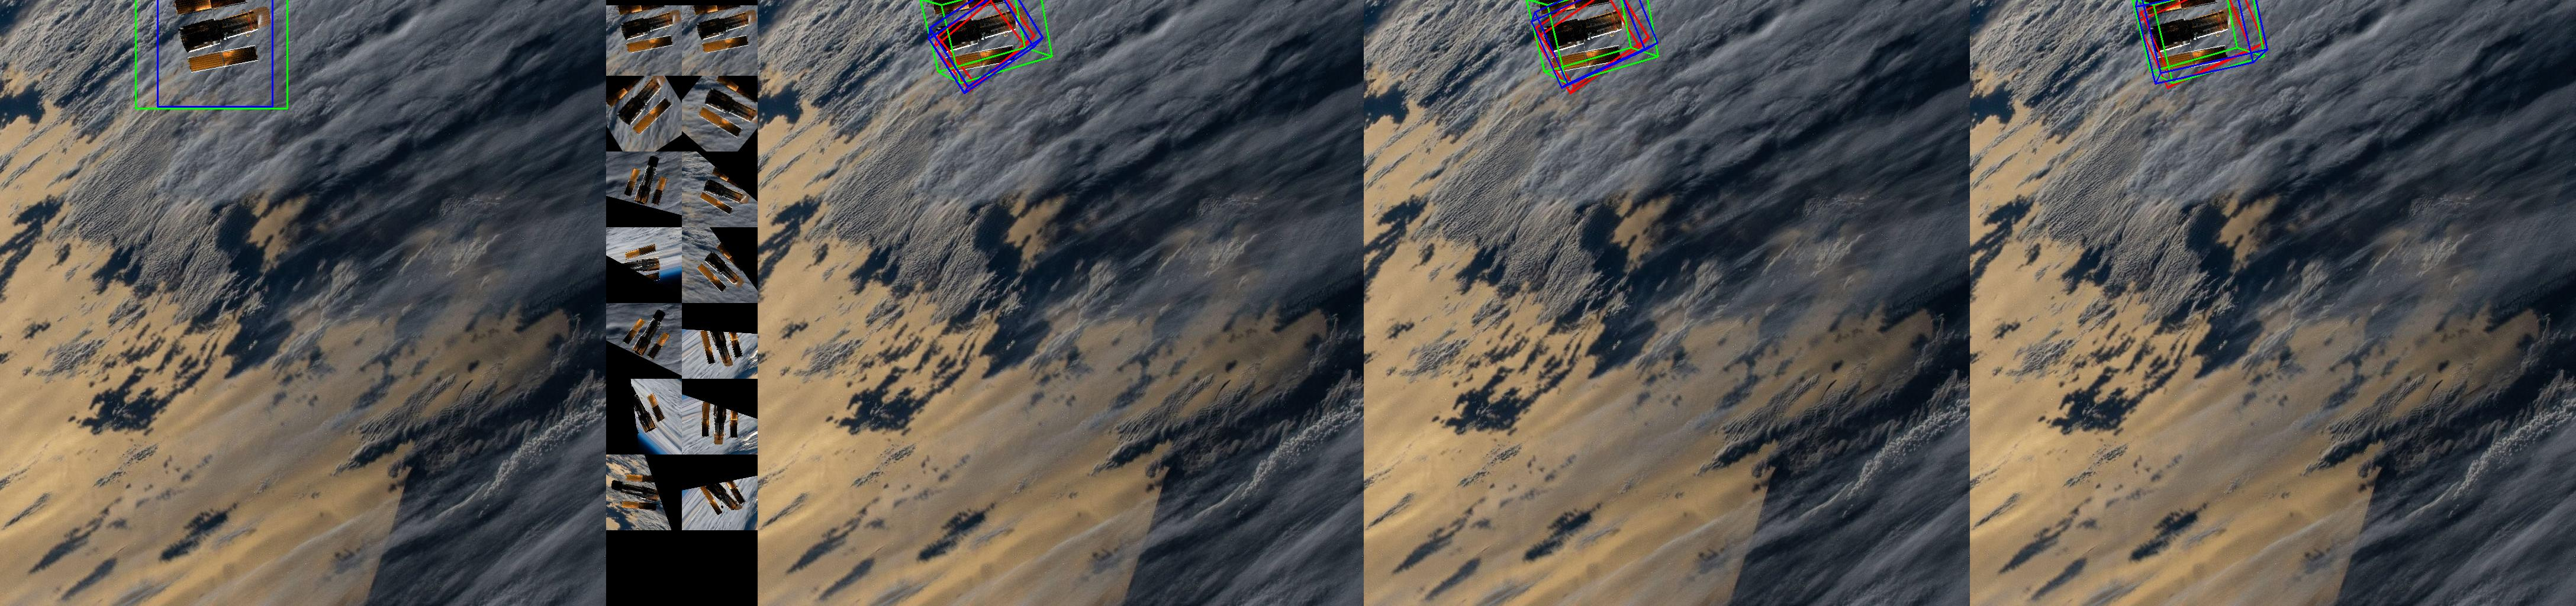
\includegraphics[width=\textwidth]{data/res1.jpg}
  \caption{An Estimation by Gen6D (Highlighted in Blue) of the Hubble Object, Presented With a Background.}
  \label{fig:cap2}
\end{figure}




%\begin{titlepage}
  \centering

  \IfFileExists{logos/tum-\fg.pdf}{%
    \includegraphics[height=20mm]{logos/tum-\fg.pdf}
  }{%
    \vspace*{20mm}
  }

  \vspace{5mm}
  {\huge\MakeUppercase{School of \getSchool{} --- \getFaculty{}} \par}

  \vspace{5mm}
  {\large\MakeUppercase{\getUniversity{}} \par}

  \vspace{20mm}
  {\Large \getDoctype{} in \getDegree{} \par}

  \vspace{15mm}
  {\huge\bfseries \getTitle{} \par}

  \vspace{10mm}
  {\huge\bfseries \foreignlanguage{ngerman}{\getTitleGer{}} \par}

  \vspace{15mm}
  \begin{tabular}{l l}
    Author:          & \getAuthor{}         \\
    Supervisor:      & \getSupervisor{}     \\
    Advisor:         & \getAdvisor{}        \\
    Submission Date: & \getSubmissionDate{} \\
  \end{tabular}

  \IfFileExists{logos/faculty-\fg.pdf}{%
    \vfill{}
    \includegraphics[height=20mm]{logos/faculty-\fg.pdf}
  }{}
\end{titlepage}

\thispagestyle{empty}
\vspace*{0.8\textheight}
\noindent
I confirm that this \MakeLowercase{\getDoctype{}} is my own work and I have documented all sources and material used.

\vspace{15mm}
\noindent
\getSubmissionLocation{}, \getSubmissionDate{} \hspace{50mm} \getAuthor{}

\cleardoublepage{}

\addcontentsline{toc}{chapter}{Acknowledgments}
\thispagestyle{empty}

\vspace*{20mm}

\begin{center}
    {\usekomafont{sectioning}\usekomafont{section}\textbf{\large Acknowledgments} }
\end{center}

%\vspace{10mm}

%TODO: Acknowledgments

\noindent Before delving into the topic, I'd like to express some acknowledgments. First and foremost I must thank my advisors Andrew Price and Chen Zhao for accepting my request to take part in a semester project under their guidance. I am grateful to have been able to practice my skills with them, and can only hope that the feeling is mutual. Moreover I would also like to thoroughly thank my friends and family for supporting me in my academic journey, despite a rather unstable start in my studies.

\cleardoublepage{}

%\chapter{\abstractname}

\addcontentsline{toc}{chapter}{Abstract}
%\thispagestyle{empty}

\vspace*{20mm}

\begin{center}
    {\usekomafont{sectioning}\usekomafont{section}\textbf{\large \abstractname} }
\end{center}

%TODO: Abstract
\microtypesetup{protrusion=false}
\tableofcontents{}
\microtypesetup{protrusion=true}

\mainmatter{}

% !TeX root = ../main.tex
% Add the above to each chapter to make compiling the PDF easier in some editors.

\chapter{Introduction}\label{chapter:introduction}

\section{Problem statement}
\subsection{The settings}
\subsection{The goal}
\section{The work environment: Scitas Izar}
% !TeX root = ../main.tex
% Add the above to each chapter to make compiling the PDF easier in some editors.

\chapter{Gen6D: Formal Description}\label{chapter:gen6d_formal_description}

\section{Overview of the Network}
After conducting a scientific literature search, we decided on an interesting model known as Gen6D: Generalizable Model-Free 6-\ac{DoF} Object Pose Estimation from RGB Images \cite{liu2023gen6d}. This architecture is fed with reference and query images, and operates in a relatively straightforward manner, comprising three stages shown in Figure~\ref{fig:fig0}. Initially, there's the detector, which, as its name suggests, detects the object in the query image. Next is the viewpoint selection, which selects reference images that have the closest viewing angle to the detected object in the query image by using a similarity score. Finally, there's the pose refiner, which enhances the accuracy of the estimated pose through a 3D volume-based process. We have compiled a table summarizing the advantages and disadvantages for a clearer understanding:

\bigskip

\begin{table}[htpb]
  \caption[Example table]{Summary of Gen6D}\label{tab:sample}
  \centering
  \small
  \begin{tabular}{l | l}
    \toprule
      Pros & Cons \\
    \midrule
      Generalizability & Limited by Reference Image Quality \\
      Model-Free & Everyday Life Objects Training Data \\
      Simple Input Requirements & Difficulty with Symmetric Objects \\
      Robustness to Background Clutter & Dependence on Initial Detection and Selection \\
      Effective in Diverse Environments & Potential Challenges with Severe Occlusions \\
      Competitive Performance & Computationally Intensive \\
    \bottomrule
  \end{tabular}
  \label{tab:tab}
\end{table}

\bigskip
\bigskip
\bigskip

\begin{figure}[ht]
  \centering
  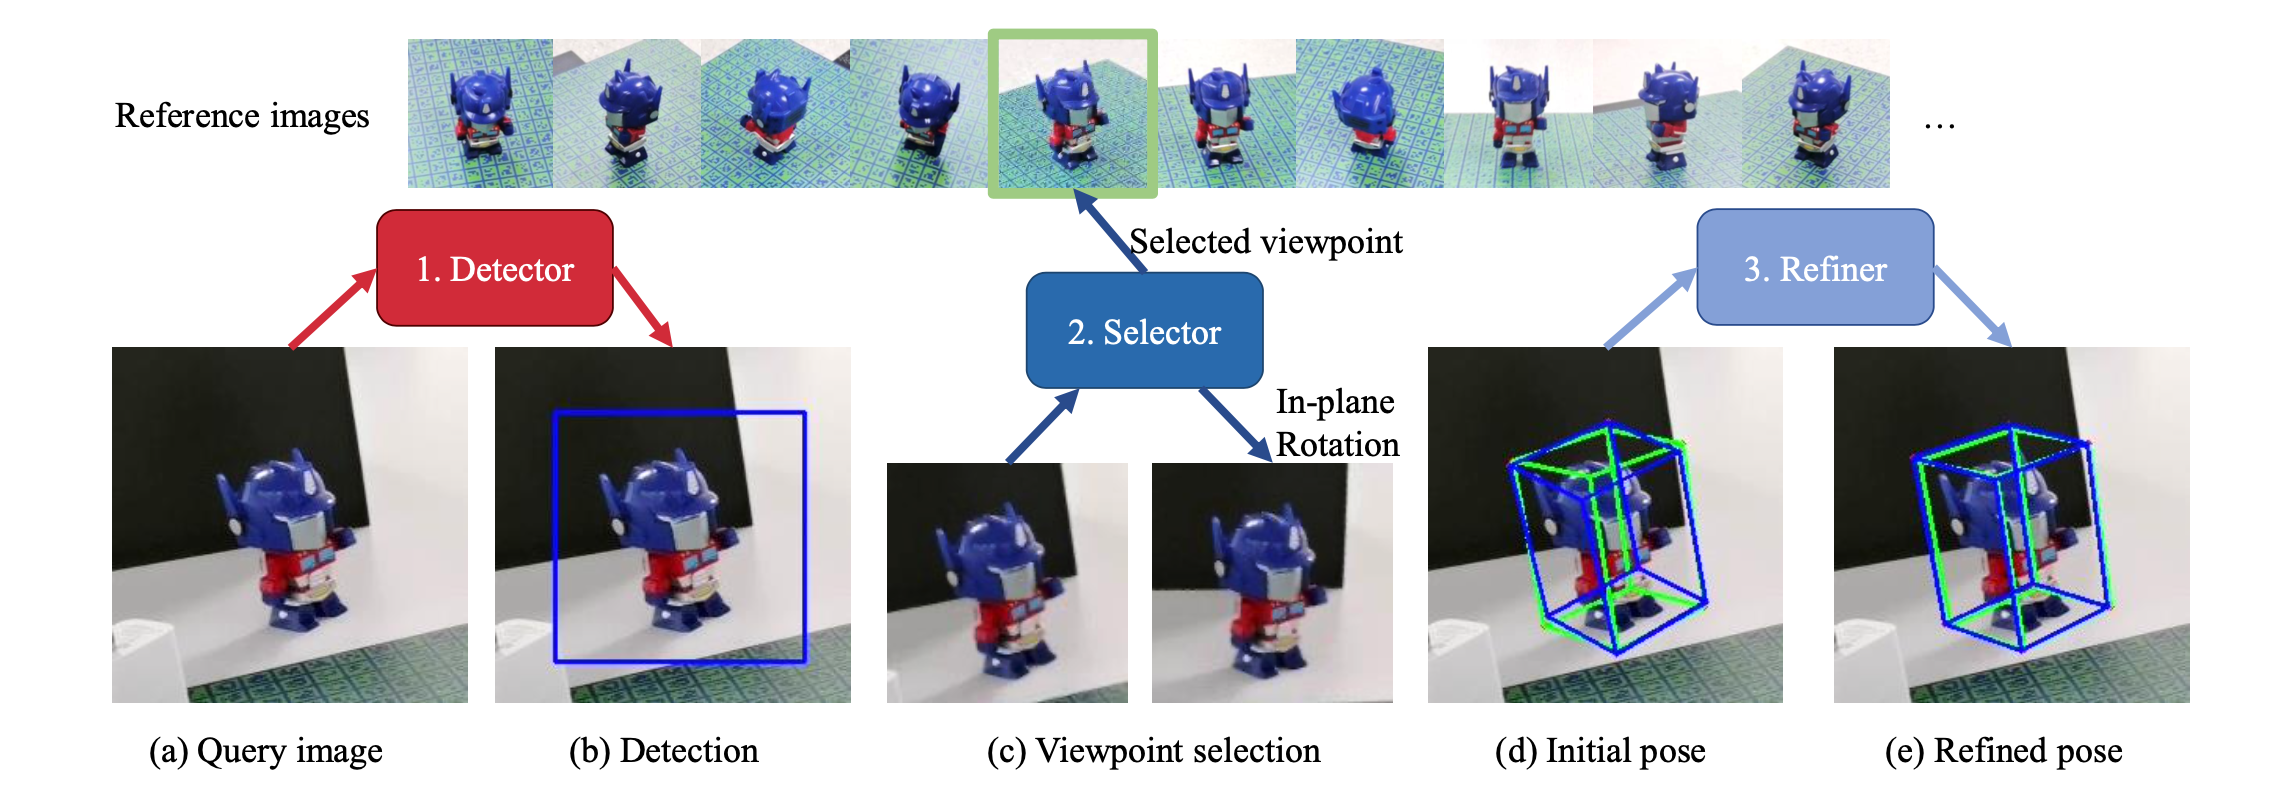
\includegraphics[width=\textwidth]{data/gen6d1.png}
  \caption{Overview of Gen6D, image sourced from Gen6D's research paper.}
  \label{fig:fig0}
\end{figure}

\cleardoublepage{}

\section{Detection}
\fancyhead[C]{\small\textsc{2.2. Detection}}

\begin{figure}[ht]
  \centering
  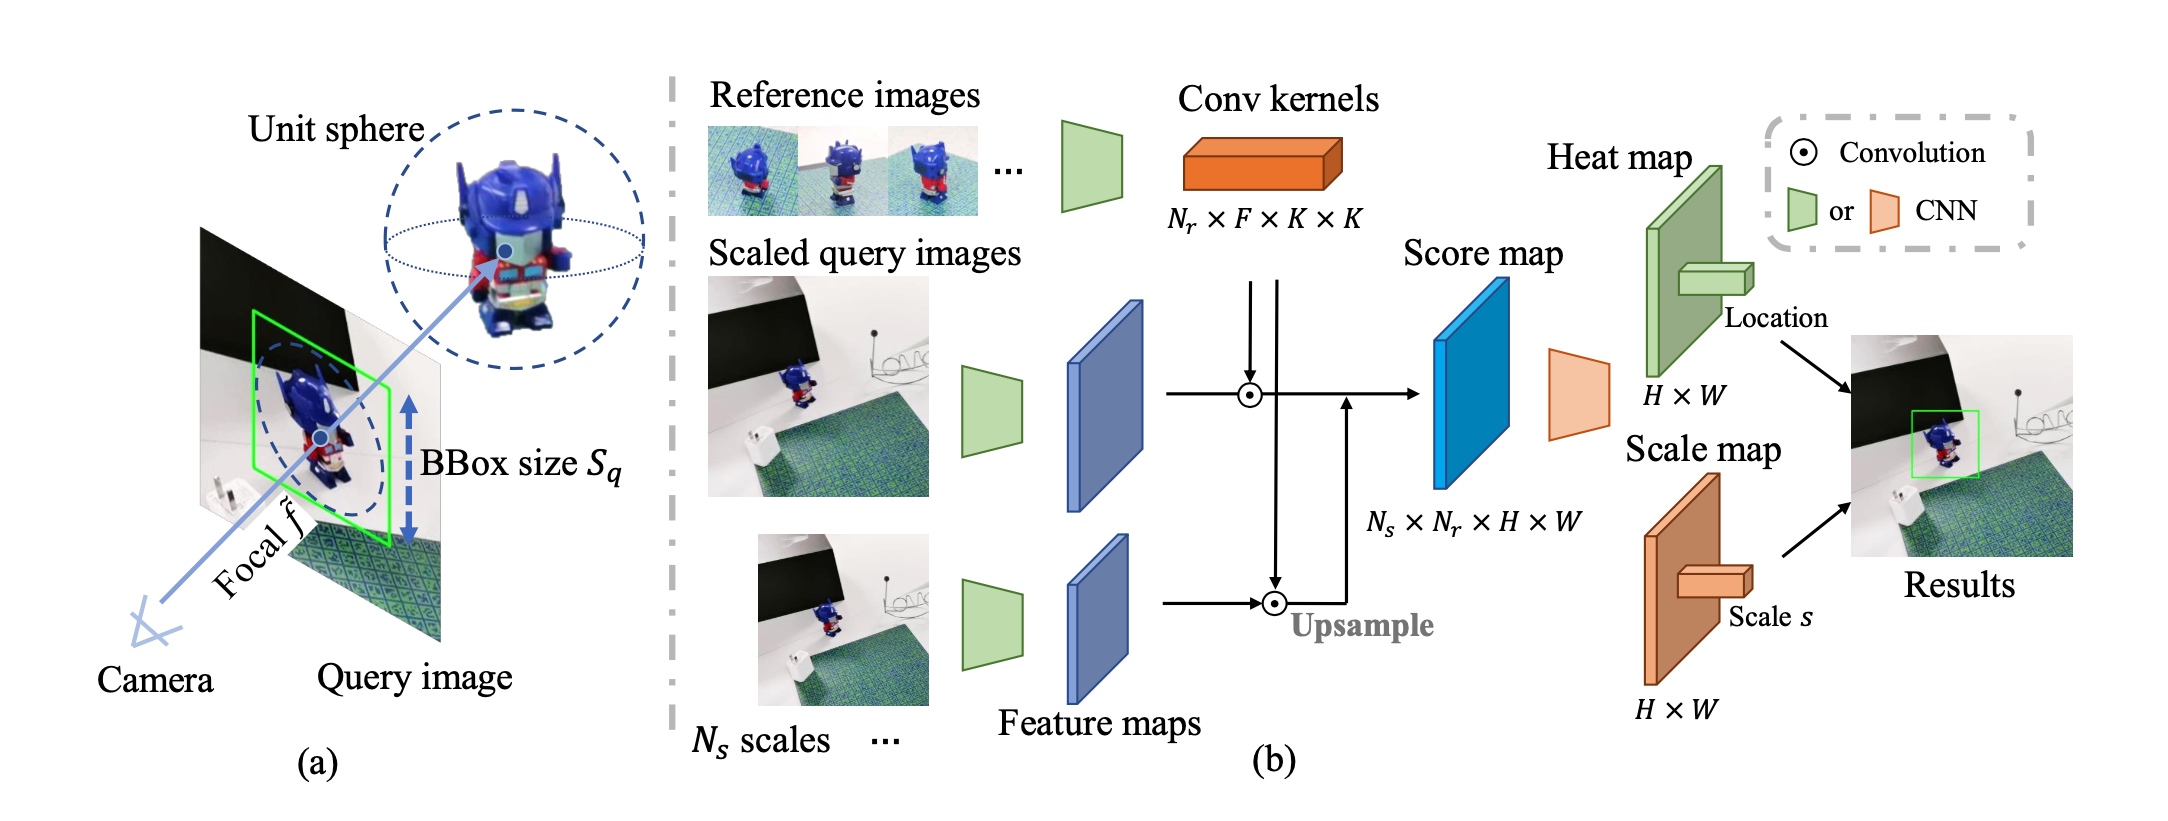
\includegraphics[width=\textwidth]{data/gen6d2.png}
  \caption{Architecture of the detector, image sourced from Gen6D's research paper.}
  \label{fig:fig1}
\end{figure}

\bigskip

In the detection phase, the initial step involves resizing both reference and query images. The reference images are resized to a dimension of $128 \times 128$, with the object centered. The query images are resized at various predefined scales. Subsequently, all the resized images are processed through a \ac{VGGNet}, which essentially functions as a deep convolutional network for extracting feature maps.

Following this, the feature maps from the reference images are utilized as convolutional kernels to convolve with one of the query images, resulting in the generation of a score map. Leveraging the multi-scale score map, we perform regression to obtain a heat map and a scale map. The final 2D detection is acquired by identifying the maximum value in the heat map, which provides the object's center coordinates, while the scale $s$ is obtained from the same location in the scale map, by this way determining the size of the 2D bounding box.

%\cleardoublepage{}

\section{Viewpoint Selection}

\begin{figure}[ht]
  \centering
  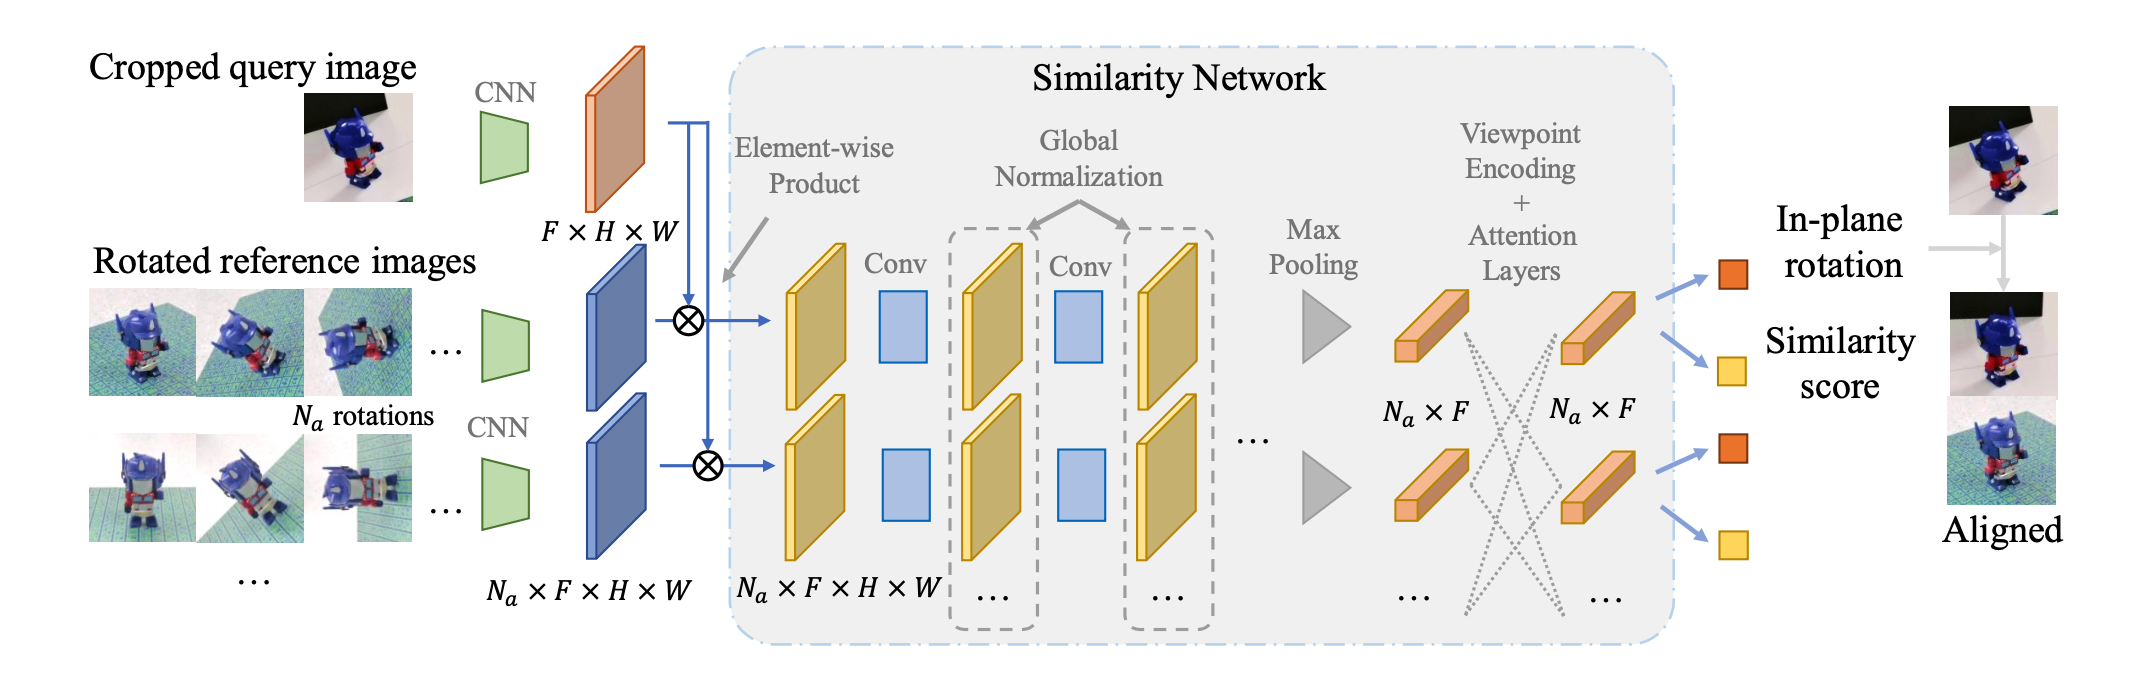
\includegraphics[width=\textwidth]{data/gen6d3.png}
  \caption{Architecture of the viewpoint selector, image sourced from Gen6D's \\ research paper.}
  \label{fig:fig2}
\end{figure}

\bigskip

During the viewpoint selection phase, we begin by applying predefined rotations to the reference images to accommodate in-plane rotation variations. After that, we once again extract feature maps from both the query image, which has been cropped based on the detection results, and the rotated reference images.

Next we calculate the element-wise product of the query image's features with those of each rotated reference image, yielding a correlation score map. These scores are then inputted into a similarity network, which produces a similarity score and the relative in-plane rotation.

It's worth highlighting that within the similarity network, the authors have implemented global normalization and incorporated a transformer to facilitate information sharing among the reference images.

\fancyhead[C]{\small\textsc{2.3. Viewpoint Selection}}


\section{Pose Refinement}

\begin{figure}[ht]
  \centering
  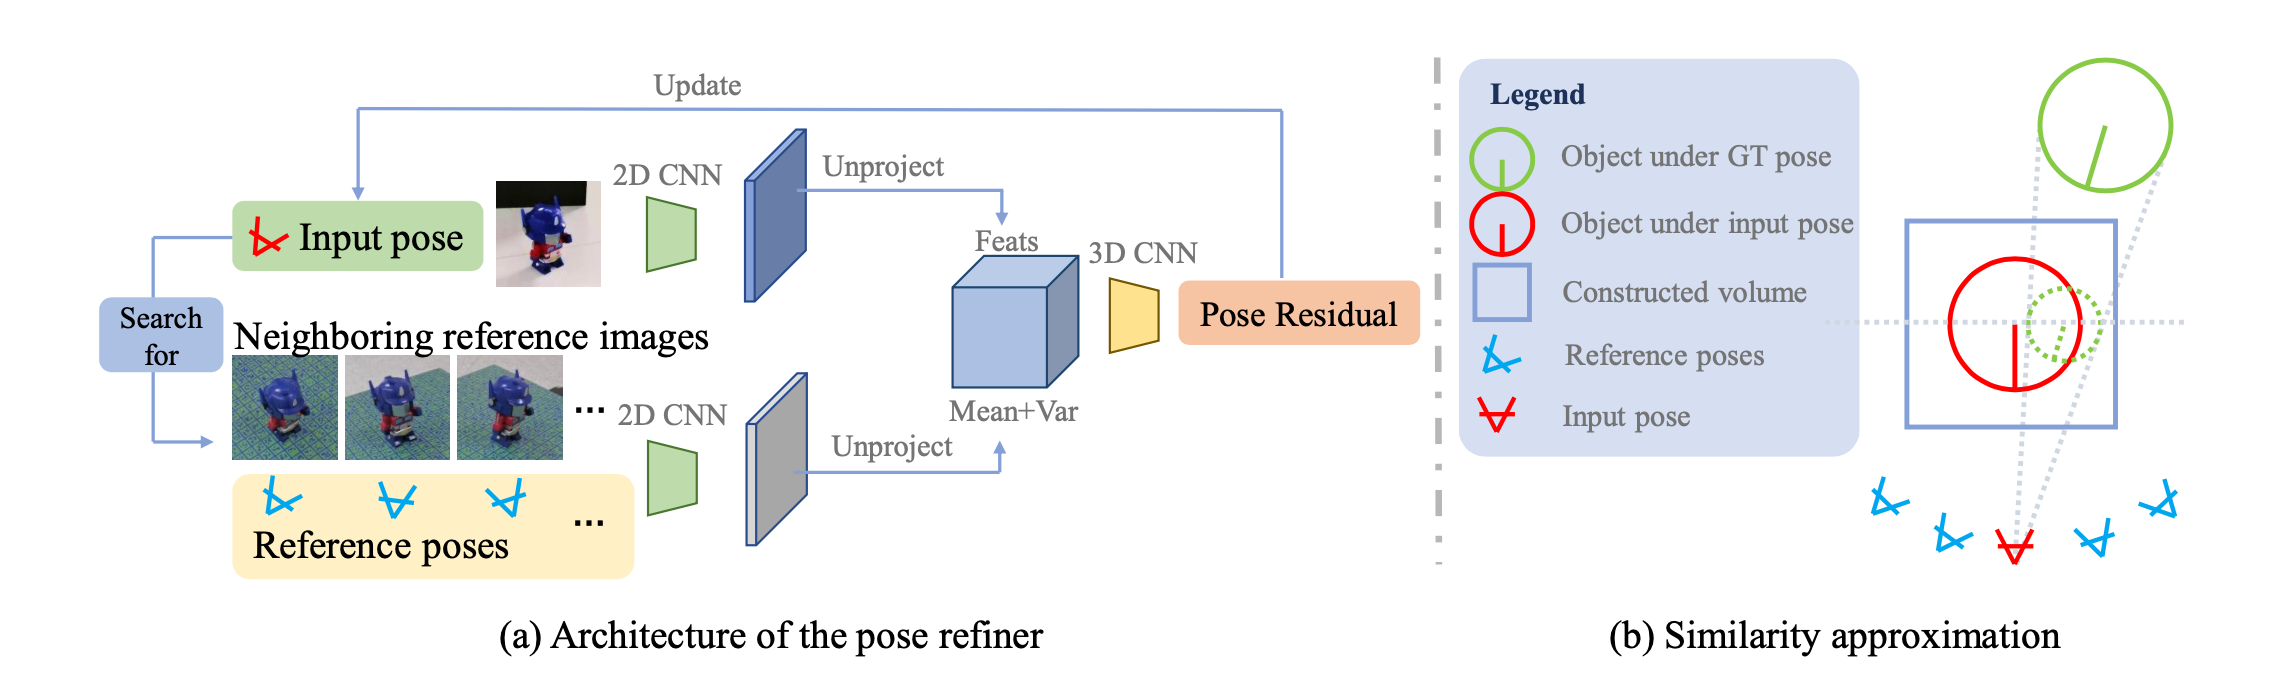
\includegraphics[width=\textwidth]{data/gen6d4.png}
  \caption{Architecture of the pose refiner, image sourced from Gen6D's research paper.}
  \label{fig:fig3}
\end{figure}

\bigskip

From the two previous stages, we have an initial coarse object pose. 
In this refinement process, we one last time extract feature maps from the selected reference images using a 2D \ac{CNN}. Afterwards, these feature maps are unprojected into the 3D volume, and we compute their mean and variance, used as features associated with the volume vertices.

Similarly, for the query image, we perform the same process but utilize the input pose. The unprojected query image features are then concatenated with the previously obtained mean and variance features.

At the end, we have a 3D \ac{CNN} that operates on the concatenated feature set of the volume, so as to predict a pose residual that updates the input pose. We iterate through the loop three times, which has been determined empirically as the optimal number of steps, in order to enhance the accuracy of the estimated pose.

%\fancyhead[C]{\small\textsc{2.4. Pose Refinement}}
% !TeX root = ../main.tex
% Add the above to each chapter to make compiling the PDF easier in some editors.

\chapter{Implementation of the model}\label{chapter:implementation_of_the_model}

\section{Data Loader}

Now that we have a better understanding of how Gen6D operates, we're interested in testing it with the synthetic images from the \textsc{Spacecraft} dataset. To accomplish this, we need to redefine the \textit{data loader} to supply the model with the necessary data in the required format. In the file \texttt{database.py}, located in the \texttt{Gen6D/dataset} directory, there is an \ac{ABC} named \texttt{BaseDatabase()} containing all the essential methods, as shown in the code below:

\bigbreak

\begin{lstlisting}[style=pythonstyle, label=lst:0, caption={Python code of \ac{ABC} \texttt{BaseDatabase()}, from file \texttt{database.py}.}]
	class BaseDatabase(abc.ABC):
    def __init__(self, database_name):
        self.database_name = database_name

    @abc.abstractmethod
    def get_image(self, img_id):
        pass

    @abc.abstractmethod
    def get_K(self, img_id):
        pass

    @abc.abstractmethod
    def get_pose(self, img_id):
        pass

    @abc.abstractmethod
    def get_img_ids(self):
        pass

    def get_mask(self,img_id):
        # dummy mask
        img = self.get_image(img_id)
        h, w = img.shape[:2]
        return np.ones([h,w],np.bool_)
\end{lstlisting}

\bigbreak

Our goal, therefore, is to write a new class that inherits from the \ac{ABC} \\\texttt{BaseDatabase()}, and implement each abstract method in the same manner as it was done for example with the \textsc{Linemod} and \textsc{GenMOP} datasets. We will also adapt the code in various places, especially in the \texttt{eval.py} file, to ensure compatibility with the \textsc{Spacecraft} dataset. The Python code for the new data loading class \texttt{SpaceCraftCVLabDatabase()} can be found in Listing~\ref{lst:1}.

\section{From Quaternions to Rotation Matrices}
\fancyhead[C]{\small\textsc{3.2. From Quaternions to Rotation Matrices}}

In Gen6D, the model represents the ground truth and estimated poses using the format ${\bm{\mathrm{P}}}=(\bm{\mathrm{R}},\,\bm{\mathrm{t}})$. Here, $\bm{\mathrm{R}}$ denotes the rotation matrix and $\bm{\mathrm{t}}$ is the translation vector.
The thing is, in the \textsc{Spacecraft} dataset, the poses have the format ${\bm{\mathrm{P}}}=(\underline{\bm{\mathrm{q}}},\,\bm{\mathrm{t}})$, where $\underline{\bm{\mathrm{q}}}$ is a \textit{quaternion}. We use quaternions for three-dimensional rotation calculations because they offer several benefits over rotation matrices. Notably, quaternions are more compact, requiring only four elements to be stored compared to nine for a matrix. Additionally, they are more efficient when composing rotations thanks to their algebraic properties.

Despite the benefits of quaternions mentioned earlier, other datasets frequently represent poses using a combination of rotation matrices and translation vectors. Therefore, to align with Gen6D's pose format, this section will focus on converting quaternions into rotation matrices \cite{jia2022quaternions}.

\bigbreak 

Quaternions were first introduced by the Irish mathematician W. R. Hamilton in 1843 as an extension of the complex numbers \cite{Hamilton1866}. In the first place, we provide the definition of a \textit{quaternion} $\underline{\bm{\mathrm{q}}}$: it is the sum of a scalar $\mathrm{q}_0$ and a vector $\bm{\mathrm{q}}=(\mathrm{q}_1, \mathrm{q}_2, \mathrm{q}_3)$, that is,
\begin{center}
	$\underline{\bm{\mathrm{q}}} \stackrel{\text{def.}}{=} \mathrm{q}_0 + \bm{\mathrm{q}} = \mathrm{q}_0 + \mathrm{q}_1\bm{i} + \mathrm{q}_2\bm{j} + \mathrm{q}_3\bm{k}$.
\end{center}

\noindent In the above, $\bm{i}$, $\bm{j}$ and $\bm{k}$ denote the three unit vectors of the canonical basis for 
the set of all ordered triples of real numbers $\mathbb{R}^3$. The set of quaternions is denoted by the 4-space $\mathbb{H}$.

\bigbreak 
The quaternion addition is component-wise. Regarding the product of two quaternions, it is essential to first outline the foundational rule established by \mbox{Hamilton}:
\begin{align*}
	\bm{i}^2 &= \bm{j}^2 = \bm{k}^2 = \bm{ijk}= -1.
\end{align*}

\noindent We derive the following multiplication table:

\begin{center}
\setlength{\arrayrulewidth}{1pt}
\renewcommand{\arraystretch}{1.2}
\begin{tabular}{|m{1.5em}||m{1.5em}|m{1.5em}|m{1.5em}|m{1.5em}|}
    \hline
    \rowcolor{gray!25}
    \cellcolor{gray!60}$\times$ & \centering $1$ & \centering $\bm{i}$ & \centering $\bm{j}$ & \centering $\bm{k}$ \tabularnewline
    \hline\hline
    \cellcolor{gray!25}$1$ & \centering $1$ & \centering $\bm{i}$ & \centering $\bm{j}$ & \centering $\bm{k}$ \tabularnewline
    \hline
    \cellcolor{gray!25}$\bm{i}$ & \centering $\bm{i}$ & \centering $-1$ & \centering $\bm{k}$ & \centering $-\bm{j}$ \tabularnewline
    \hline
    \cellcolor{gray!25}$\bm{j}$ & \centering $\bm{j}$ & \centering $-\bm{k}$ & \centering $-1$ & \centering $\bm{i}$ \tabularnewline
    \hline
    \cellcolor{gray!25}$\bm{k}$ & \centering $\bm{k}$ & \centering $\bm{j}$ & \centering $-\bm{i}$ & \centering $-1$ \tabularnewline
    \hline
\end{tabular}
\end{center}

% TABLE FOR DARK JOB
%\begin{center}
%\setlength{\arrayrulewidth}{1pt}
%\renewcommand{\arraystretch}{1.2}
%\begin{tabular}{|m{1.5em}||m{1.5em}|m{1.5em}|m{1.5em}|m{1.5em}|}
%    \hline
%    $\times$ & \centering $1$ & \centering $\bm{i}$ & \centering $\bm{j}$ & \centering $\bm{k}$ \tabularnewline
%    \hline\hline
%    $1$ & \centering $1$ & \centering $\bm{i}$ & \centering $\bm{j}$ & \centering $\bm{k}$ \tabularnewline
%    \hline
%    $\bm{i}$ & \centering $\bm{i}$ & \centering $-1$ & \centering $\bm{k}$ & \centering $-\bm{j}$ \tabularnewline
%    \hline
%    $\bm{j}$ & \centering $\bm{j}$ & \centering $-\bm{k}$ & \centering $-1$ & \centering $\bm{i}$ \tabularnewline
%    \hline
%    $\bm{k}$ & \centering $\bm{k}$ & \centering $\bm{j}$ & \centering $-\bm{i}$ & \centering $-1$ \tabularnewline
%    \hline
%\end{tabular}
%\end{center}

\bigbreak 

\noindent Let $(\underline{\bm{\mathrm{p}}}, \underline{\bm{\mathrm{q}}})\in\mathbb{H}^2$, we are now able to present the multiplication of $\underline{\bm{\mathrm{p}}}$ and $\underline{\bm{\mathrm{q}}}$:
\begin{align*}
    \underline{\bm{\mathrm{p}}}\underline{\bm{\mathrm{q}}} &= \underbrace{\mathrm{p}_0\mathrm{q}_0 - \bm{\mathrm{p}} \cdot \bm{\mathrm{q}}}_{\text{scalar part}} + \underbrace{\mathrm{p}_0\bm{\mathrm{q}} + \mathrm{q}_0\bm{\mathrm{p}} + \bm{\mathrm{p}} \times \bm{\mathrm{q}}}_{\text{vector part}}.
\end{align*}

\noindent In the preceding, we recall that the binary operation $\mathbb{R}^3\times\mathbb{R}^3\rightarrow\mathbb{R}$ : $(\bm{\mathrm{p}},\bm{\mathrm{q}})\mapsto\bm{\mathrm{p}}\cdot\bm{\mathrm{q}}\stackrel{\text{def.}}{=}\bm{\mathrm{p}}^\intercal\bm{\mathrm{q}}$ is the \textit{dot product}, and the other
\begin{align*}
	\mathbb{R}^3\times\mathbb{R}^3\rightarrow\mathbb{R}^3 : (\bm{\mathrm{p}},\bm{\mathrm{q}})\mapsto\bm{\mathrm{p}}\times\bm{\mathrm{q}}\stackrel{\text{def.}}{=}\begin{vmatrix} \bm{i} & \bm{j} & \bm{k} \\ \mathrm{p}_1 & \mathrm{p}_2 & \mathrm{p}_3 \\
		\mathrm{q}_1 & \mathrm{q}_2 & \mathrm{q}_3 \end{vmatrix}
		=[\bm{\mathrm{p}}]_{_{_\times}}\bm{\mathrm{q}}
\end{align*}

\noindent is the \textit{cross product}, and the operator $[\bm{\mathrm{p}}]_{_{_\times}}$yields the transformation matrix that when multiplied from the right with a vector $\bm{\mathrm{q}}$ gives $\bm{\mathrm{p}}\times\bm{\mathrm{q}}$.
\bigbreak 
Several additional definitions are essential before we can begin the conversion of quaternions to rotation matrices. 


\noindent Let $\underline{\bm{\mathrm{q}}}=\mathrm{q}_0 + \bm{\mathrm{q}}$ be a quaternion. The \textit{complex conjugate} of $\underline{\bm{\mathrm{q}}}$, denoted by $\underline{\bm{\mathrm{q}}}^\star$, is given by the map
\begin{align*}
	\mathbb{H}\rightarrow\mathbb{H}:\underline{\bm{\mathrm{q}}}\mapsto\underline{\bm{\mathrm{q}}}^\star\stackrel{\text{def.}}{=}\mathrm{q}_0 - \bm{\mathrm{q}}.
\end{align*} 

\noindent The \textit{norm} of a quaternion $\underline{\bm{\mathrm{q}}}$, denoted $|\underline{\bm{\mathrm{q}}}|$, is the distance obtained from the map 
\begin{align*}
	\mathbb{H}\rightarrow\mathbb{R}^+:\underline{\bm{\mathrm{q}}}\mapsto|\underline{\bm{\mathrm{q}}}|\stackrel{\text{def.}}{=}\sqrt{\underline{\bm{\mathrm{q}}}^\star\underline{\bm{\mathrm{q}}}}.
\end{align*} 
Note that a quaternion whose norm is 1 is referred to as a \textit{unit quaternion}. The \textit{reciprocal} of a quaternion is defined as the map
\begin{align*}
	\mathbb{H}^*\rightarrow\mathbb{H}^*:\underline{\bm{\mathrm{q}}}\mapsto\underline{\bm{\mathrm{q}}}^{-1}\stackrel{\text{def.}}{=}\frac{\underline{\bm{\mathrm{q}}}^\star}{|\underline{\bm{\mathrm{q}}}|^2}.
\end{align*} 
We observe that if $\underline{\bm{\mathrm{q}}}$ is a unit quaternion, we simply have $\underline{\bm{\mathrm{q}}}^{-1}=\underline{\bm{\mathrm{q}}}^\star$. Furthermore, the subsequent proposition is accepted: if $\underline{\bm{\mathrm{q}}}$ is a unit quaternion, there exists a unique $\theta\in[0,2\pi]$ such that
\begin{align*}
	\underline{\bm{\mathrm{q}}} = \mathrm{q}_0 + \bm{\mathrm{q}}=\cos\frac{\theta}{2}+\bm{\mathrm{u}}\,\sin\frac{\theta}{2}\,,
\end{align*}
where the unit vector $\bm{\mathrm{u}}$ is defined as $\bm{\mathrm{u}}\stackrel{\text{def.}}{=}\frac{\bm{\mathrm{q}}}{|\bm{\mathrm{q}}|}$.

\setlength{\belowdisplayskip}{0.15cm}

\paragraph{Quaternion Rotation Operator} Let $\underline{\bm{\mathrm{q}}}\in\mathbb{H}$ be a unit quaternion, and let $\bm{\mathrm{v}}\in\mathbb{R}^3$ be a vector. The action of the $L_{\underline{\bm{\mathrm{q}}}}$ function 
\begin{align*}
	\mathbb{R}^3\rightarrow\mathbb{R}^3:\bm{\mathrm{v}}\mapsto L_{\underline{\bm{\mathrm{q}}}}(\bm{\mathrm{v}}) \stackrel{\text{def.}}{=} \underline{\bm{\mathrm{q}}}\bm{\mathrm{v}}\underline{\bm{\mathrm{q}}}^\star
\end{align*}
on $\bm{\mathrm{v}}$ is equivalent to a rotation of the vector through an angle $\theta$ about the axis of rotation $\bm{\mathrm{u}}$.

\setlength{\belowdisplayskip}{0.3cm}

\bigskip
\bigskip 

At last, we can proceed with our conversion task: our aim is to find a $3\times3$ rotation matrix $\bm{\mathrm{R}}$, such that
\begin{align*}
\left\{
    \begin{aligned}
    	L_{\bm{\mathrm{R}}}(\bm{\mathrm{v}}) &\stackrel{\text{def.}}{=} \bm{\mathrm{R}}\bm{\mathrm{v}} \\
        L_{\bm{\mathrm{R}}}(\bm{\mathrm{v}}) &= L_{\underline{\bm{\mathrm{q}}}}(\bm{\mathrm{v}}),
    \end{aligned}
\right.
\end{align*}

\noindent which means we wish to obtain an expression for $\bm{\mathrm{R}}$ by manipulating $L_{\underline{\bm{\mathrm{q}}}}\,$, utilizing principles of linear algebra and vector calculus. We consider the vector $\bm{\mathrm{v}}$ as a quaternion with a zero scalar component:

\begin{align*}
    L_{\underline{\bm{\mathrm{q}}}}(\bm{\mathrm{v}}) &= \underline{\bm{\mathrm{q}}}\bm{\mathrm{v}}\underline{\bm{\mathrm{q}}}^\star \\
    &= (\mathrm{q}_0+\bm{\mathrm{q}})(0+\bm{\mathrm{v}})(\mathrm{q}_0-\bm{\mathrm{q}}) \\
    &= (\underbrace{-\bm{\mathrm{q}}\cdot\bm{\mathrm{v}}}_{\text{scalar part}} + \underbrace{\mathrm{q}_0\bm{\mathrm{v}}+\bm{\mathrm{q}}\times\bm{\mathrm{v}}}_{\text{vector part}})(\mathrm{q}_0-\bm{\mathrm{q}}) \\
    &= \mathrm{q}_0(-\bm{\mathrm{q}}\cdot\bm{\mathrm{v}}) - (\mathrm{q}_0\bm{\mathrm{v}}+\bm{\mathrm{q}}\times\bm{\mathrm{v}})\cdot(-\bm{\mathrm{q}}) \\
    &\quad + (-\bm{\mathrm{q}}\cdot\bm{\mathrm{v}})(-\bm{\mathrm{q}}) + \mathrm{q}_0(\mathrm{q}_0\bm{\mathrm{v}}+\bm{\mathrm{q}}\times\bm{\mathrm{v}}) \\
    &\quad + (\mathrm{q}_0\bm{\mathrm{v}}+\bm{\mathrm{q}}\times\bm{\mathrm{v}})\times(-\bm{\mathrm{q}}) \\
    &= \underbrace{\cancel{-\mathrm{q}_0(\bm{\mathrm{q}}\cdot\bm{\mathrm{v}}) + \mathrm{q}_0(\bm{\mathrm{q}}\cdot\bm{\mathrm{v}})}}_{\text{scalar part}} \\
    &\quad + \underbrace{\bm{\mathrm{q}}\,(\bm{\mathrm{q}}\cdot\bm{\mathrm{v}}) + {\mathrm{q}_0}^2\,\bm{\mathrm{v}} + \mathrm{q}_0(\bm{\mathrm{q}}\times\bm{\mathrm{v}}) + \bm{\mathrm{q}}\times(\mathrm{q}_0\bm{\mathrm{v}}+\bm{\mathrm{q}}\times\bm{\mathrm{v}})}_{\text{vector part}} \\
    &= \bm{\mathrm{q}}\,(\bm{\mathrm{q}}^\intercal\bm{\mathrm{v}}) + {\mathrm{q}_0}^2\,\bm{\mathrm{v}} + \mathrm{q}_0(\bm{\mathrm{q}}\times\bm{\mathrm{v}}) + \bm{\mathrm{q}}\times(\mathrm{q}_0\bm{\mathrm{v}}+\bm{\mathrm{q}}\times\bm{\mathrm{v}}) \\
    &= (\bm{\mathrm{q}}\otimes\bm{\mathrm{q}} + {\mathrm{q}_0}^2\,\bm{\mathrm{I}}_{3\times3} + 2\,\mathrm{q}_0\,[\bm{\mathrm{q}}]_{_{_\times}}\!\! + [\bm{\mathrm{q}}]_{_{_\times}}^2)\,\,\bm{\mathrm{v}}
\end{align*}

\bigskip

\noindent In the above, $\otimes$ stands for the \textit{outer product} and $\bm{\mathrm{I}}_{3\times3}$ is the \textit{identity matrix}. 

\noindent Since $L_{\bm{\mathrm{R}}}(\bm{\mathrm{v}}) = L_{\underline{\bm{\mathrm{q}}}}(\bm{\mathrm{v}})$, we can identify $\bm{\mathrm{R}}$ as  $(\bm{\mathrm{q}}\otimes\bm{\mathrm{q}} + {\mathrm{q}_0}^2\,\bm{\mathrm{I}}_{3\times3} + 2\,\mathrm{q}_0\,[\bm{\mathrm{q}}]_{_{_\times}}\!\! + [\bm{\mathrm{q}}]_{_{_\times}}^2)$. We develop and simplify $\bm{\mathrm{R}}$ to find its final expression:

\begin{align*}
	\bm{\mathrm{R}} &= \bm{\mathrm{q}}\otimes\bm{\mathrm{q}} + {\mathrm{q}_0}^2\,\bm{\mathrm{I}}_{3\times3} + 2\,\mathrm{q}_0\,[\bm{\mathrm{q}}]_{_{_\times}}\!\! + [\bm{\mathrm{q}}]_{_{_\times}}^2 \\
	&= \begin{bmatrix}
    	{\mathrm{q}_1}^2 & \mathrm{q}_1\mathrm{q}_2 & \mathrm{q}_1\mathrm{q}_3 \\
    	\mathrm{q}_2\mathrm{q}_1 & {\mathrm{q}_2}^2 & \mathrm{q}_2\mathrm{q}_3 \\
    	\mathrm{q}_3\mathrm{q}_1 & \mathrm{q}_3\mathrm{q}_2 & {\mathrm{q}_3}^2
		\end{bmatrix} 
		+ {\mathrm{q}_0}^2
		\begin{bmatrix}
    	1 & 0 & 0 \\
    	0 & 1 & 0 \\
    	0 & 0 & 1
		\end{bmatrix}
		+
		2\,\mathrm{q}_0 \begin{bmatrix}
    	0 & -\mathrm{q}_3 & \mathrm{q}_2 \\
    	\mathrm{q}_3 & 0 & -\mathrm{q}_1 \\
    	-\mathrm{q}_2 & \mathrm{q}_1 & 0
		\end{bmatrix} \\
		&\quad+
		\begin{bmatrix}
    	0 & -\mathrm{q}_3 & \mathrm{q}_2 \\
    	\mathrm{q}_3 & 0 & -\mathrm{q}_1 \\
    	-\mathrm{q}_2 & \mathrm{q}_1 & 0
		\end{bmatrix}
		\begin{bmatrix}
    	0 & -\mathrm{q}_3 & \mathrm{q}_2 \\
    	\mathrm{q}_3 & 0 & -\mathrm{q}_1 \\
    	-\mathrm{q}_2 & \mathrm{q}_1 & 0
		\end{bmatrix} \\\\
		&=2
		\begin{bmatrix}
    	({\mathrm{q}_0}^2+{\mathrm{q}_1}^2)-\frac{1}{2} & \mathrm{q}_1\mathrm{q}_2-\mathrm{q}_0\mathrm{q}_3 & \mathrm{q}_1\mathrm{q}_3+\mathrm{q}_0\mathrm{q}_2 \\
    	\mathrm{q}_1\mathrm{q}_2+\mathrm{q}_0\mathrm{q}_3 & ({\mathrm{q}_0}^2+{\mathrm{q}_2}^2)-\frac{1}{2} & \mathrm{q}_2\mathrm{q}_3-\mathrm{q}_0\mathrm{q}_1 \\
    	\mathrm{q}_1\mathrm{q}_3-\mathrm{q}_0\mathrm{q}_2 & \mathrm{q}_2\mathrm{q}_3+\mathrm{q}_0\mathrm{q}_1 & ({\mathrm{q}_0}^2+{\mathrm{q}_3}^2)-\frac{1}{2}
		\end{bmatrix}
\end{align*} 

\bigskip

\noindent This completes our derivation of the rotation matrix $\bm{\mathrm{R}}$. The Python code can be found in Listing~\ref{lst:4}.

\section{Inverted Masks}

During the initial testing of Gen6D on the \textsc{Spacecraft} dataset, we noticed that the estimated poses were particularly inaccurate. Upon investigation, we discovered that in the reference images folder, the masks were incorrectly inverted: typically, one expects a white object on a black background, but it was the opposite (see Figure~\ref{fig:mask1} below).

After discussing this, we realized that this was actually an error in the current version of the dataset. Therefore, we needed to correct the masks we were using through a Python script utilizing the OpenCV library. The Python script can be found in Listing~\ref{lst:5}.

\fancyhead[C]{\small\textsc{3.3. Inverted Masks}}

\bigskip

\begin{figure}[h]
    \centering
    \begin{minipage}{0.45\linewidth}
        \centering
        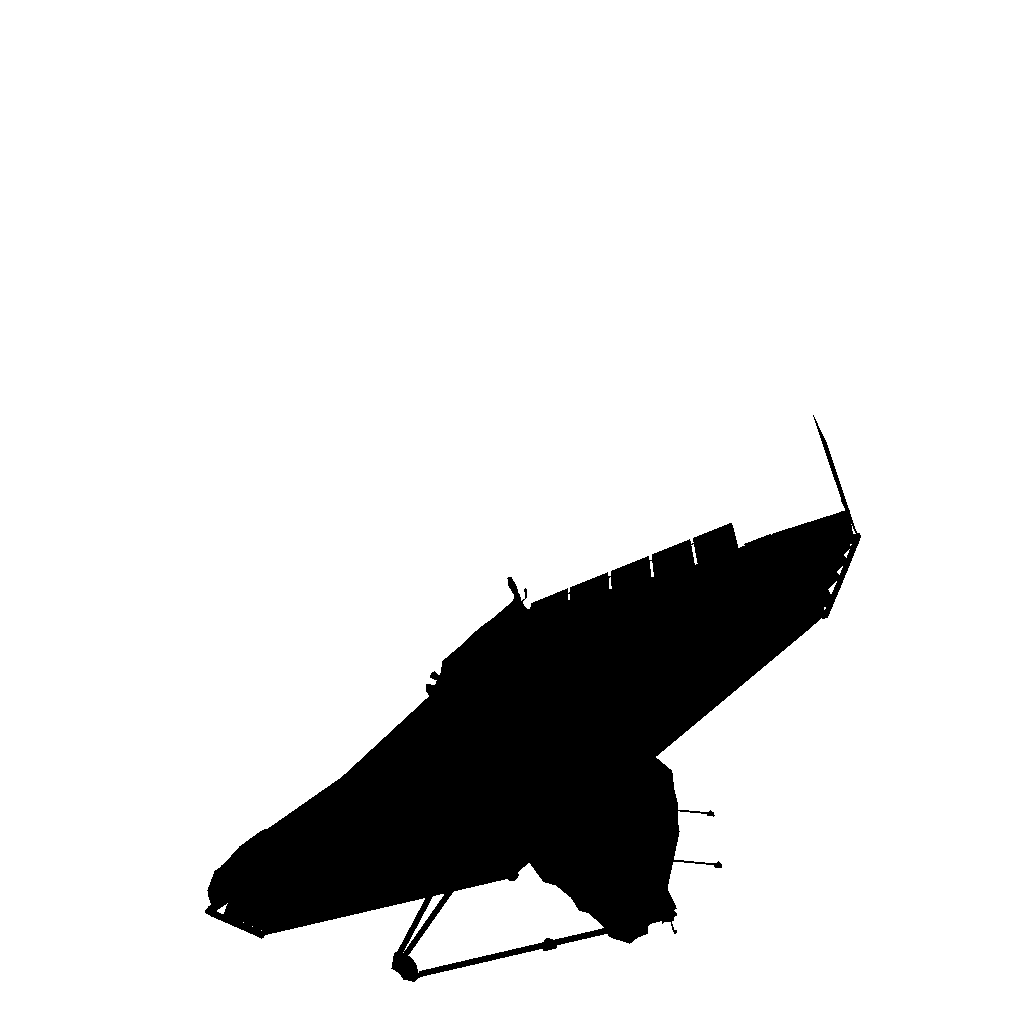
\includegraphics[width=\linewidth]{data/mask1.png} % First image
        \caption{James Webb Space Telescope, mask before the correction.}
        \label{fig:mask1}
    \end{minipage}\hfill
    \begin{minipage}{0.45\linewidth}
        \centering
        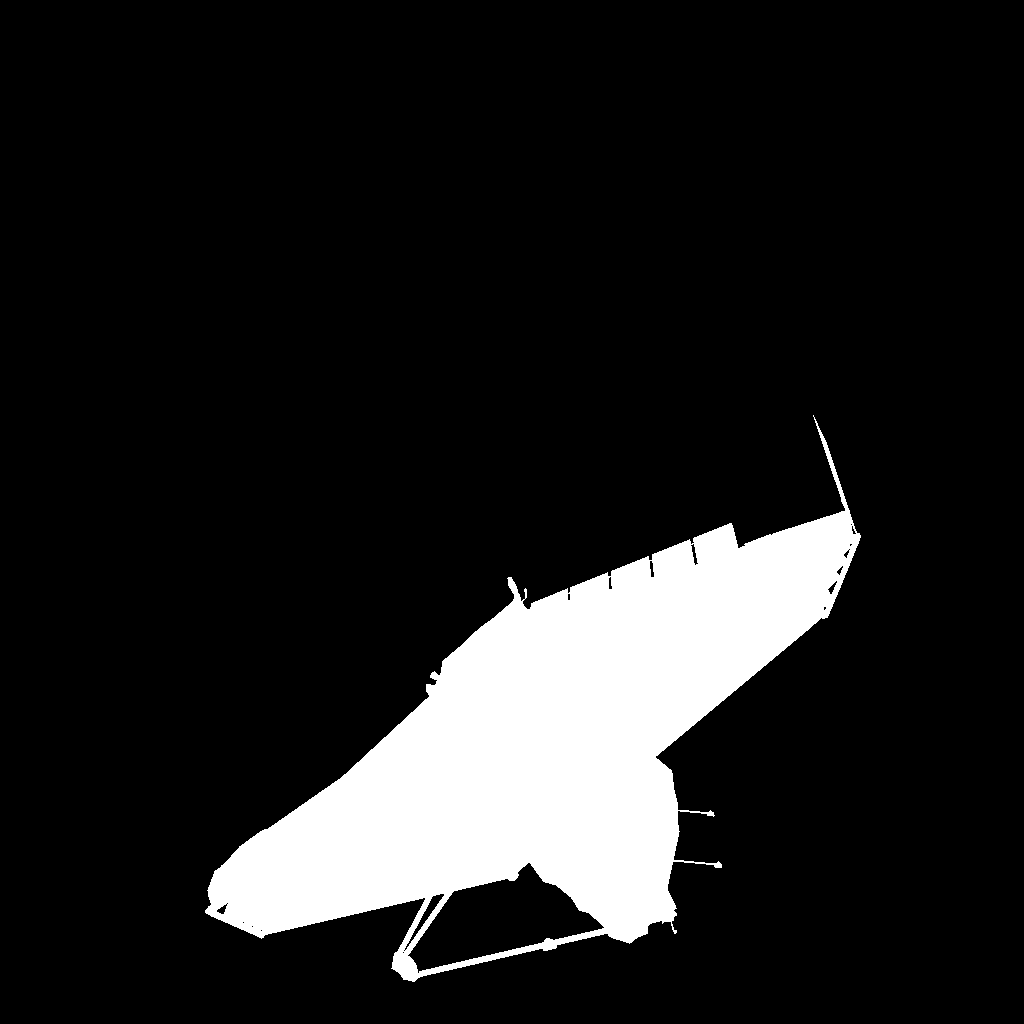
\includegraphics[width=\linewidth]{data/mask2.png} % Second image
        \caption{James Webb Space Telescope, mask after the correction using a script.}
        \label{fig:mask2}
    \end{minipage}
\end{figure}

\bigskip

\section{Resized Query Images}

During the initial testing of Gen6D, it became apparent that the deep learning model struggled when the object in the query image was either very large or very small (see Figure~\ref{fig:fig2} and Figure~\ref{fig:fig1} below). Consultation of the GitHub Issues section of the Gen6D repository revealed that this is a recurring problem: since the reference images are resized to $128\times 128$, the model's detector is trained to recognize an object in query images that ranges from half to double the size of the reference images, i.e., from $64\times 64$ to $256\times 256$.

\bigskip

Therefore, to improve the detector's results, resizing the query images is necessary. This is accomplished using a Python script that can be found in Listing~\ref{lst:6}. It's important to note that this adjustment also requires modifying the camera intrinsic matrix $\bm{\mathcal{K}}$ in the data loader, which converts points from the camera coordinate system to the pixel coordinate system.

\pagebreak

\fancyhead[C]{\small\textsc{3.4. Resized Query Images}}

\begin{figure}[H]
    \centering
    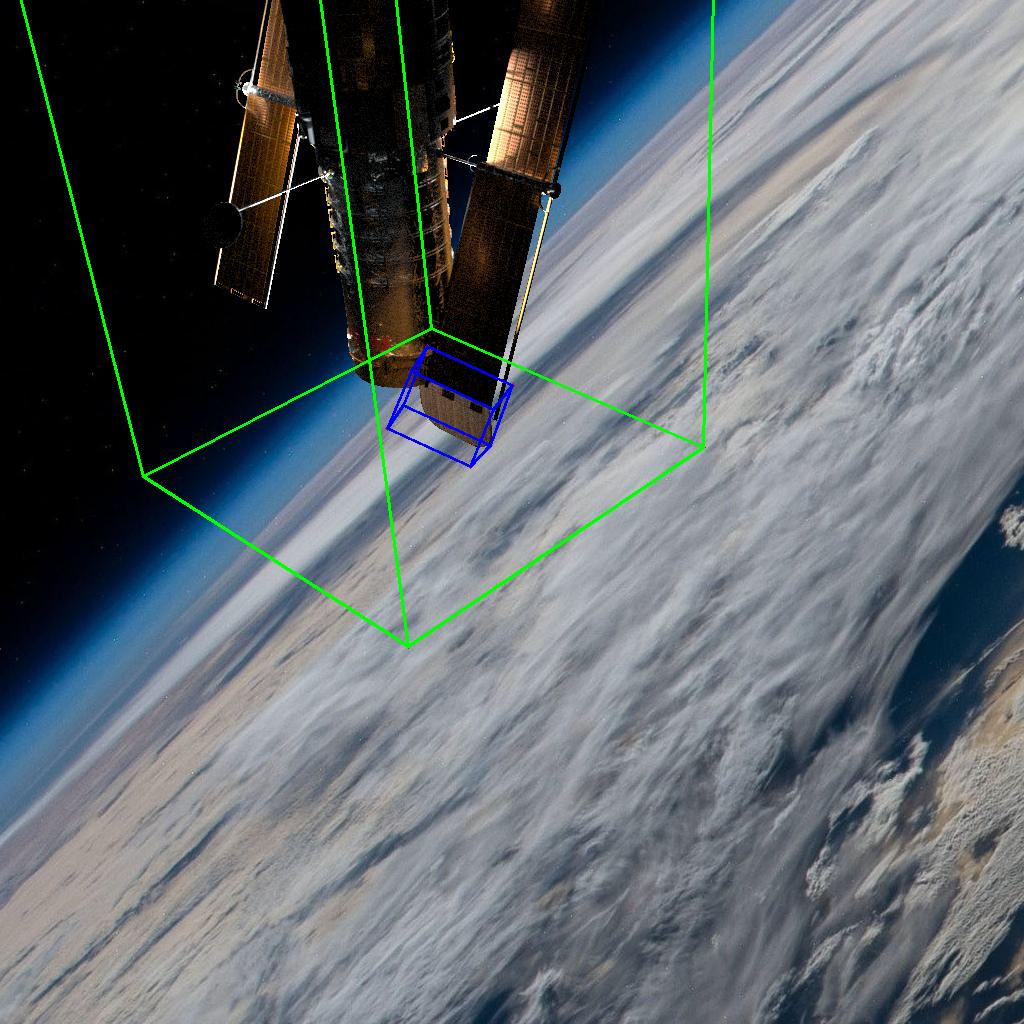
\includegraphics[width=0.70\linewidth]{data/fig2.jpg}
    \caption{Hubble Space Telescope with earth rendered background, 1024x1024 query image number 1, poor pose estimation (blue 3D bounding box) when the object inside the query image is too big.}
    \label{fig:fig2}
\end{figure}

\bigskip
\bigskip
\bigskip

\begin{figure}[H]
    \centering
    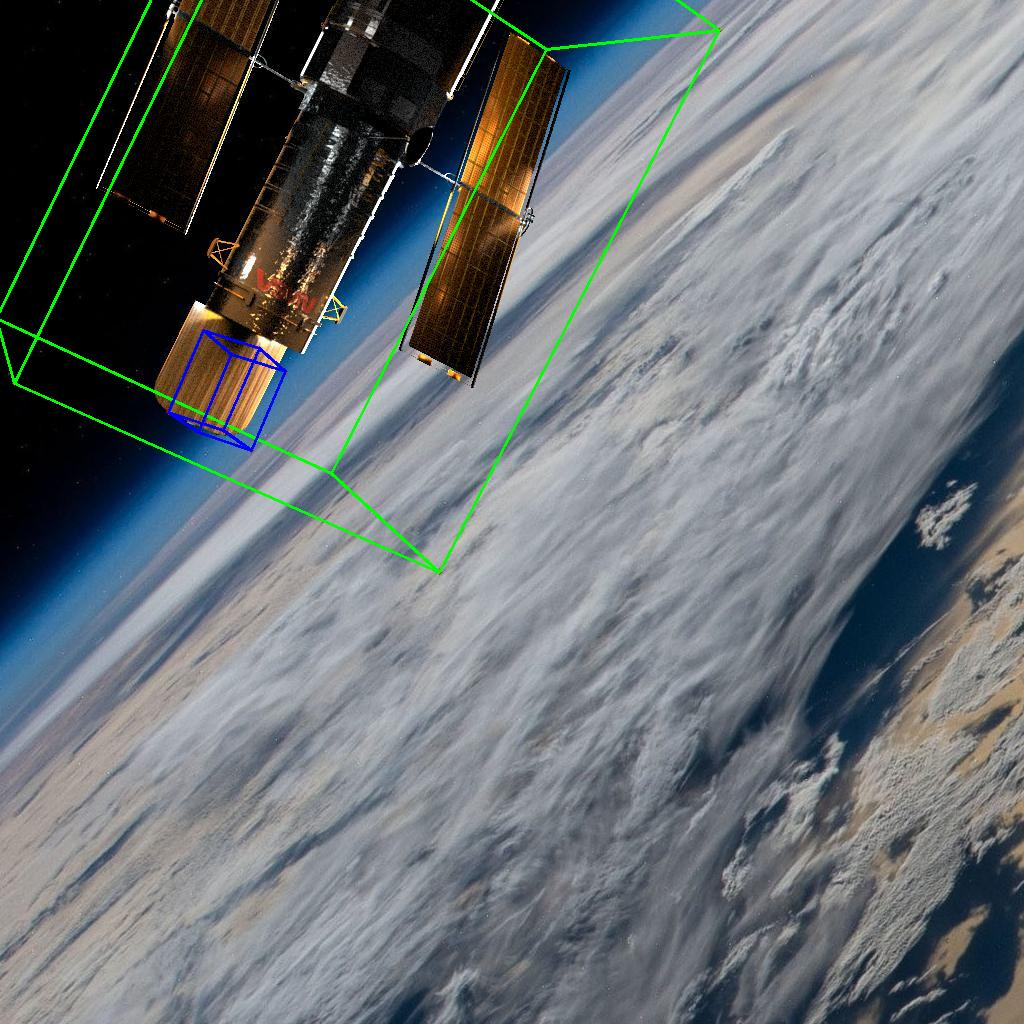
\includegraphics[width=0.70\linewidth]{data/fig1.jpg}
    \caption{Hubble Space Telescope with earth rendered background, 1024x1024 query image number 2, poor pose estimation (blue 3D bounding box) when the object inside the query image is too big.}
    \label{fig:fig1}
\end{figure}

% !TeX root = ../main.tex
% Add the above to each chapter to make compiling the PDF easier in some editors.

\chapter{Experimental Results and Analysis}\label{chapter:presentation_of_the_results}

\section{Evaluation Metrics}

To appreciate the quality of the estimations, the most widely used pose error functions are the \ac{ADD} and the \ac{ADD-S} metrics, both introduced by Hinterstoisser et al. \cite{10.1007/978-3-642-37331-2_42}. For an object model $\mathcal{M}$, we compute the average distance to the corresponding model point. Therefore the error of an estimated pose $\hat{\bm{\mathrm{P}}}=(\hat{\bm{\mathrm{R}}},\,\hat{\bm{\mathrm{t}}})$ w.r.t. the ground truth pose $\bar{\bm{\mathrm{P}}}=(\bar{\bm{\mathrm{R}}},\,\bar{\bm{\mathrm{t}}})$ is calculated as follows:

\begin{align}
	\textit{\footnotemark}e_\mathrm{ADD}(\hat{\bm{\mathrm{P}}},\,\bar{\bm{\mathrm{P}}},\,\mathcal{M})\stackrel{\text{def.}}{=}&\underset{\bm{\mathrm{x}}\in\mathcal{M}}{\mathrm{avg}}\norm\bigg{\bar{\bm{\mathrm{P}}}\bm{\mathrm{x}}^\star-\hat{\bm{\mathrm{P}}}\bm{\mathrm{x}}^\star}_2 \\
	=\,&\underset{\bm{\mathrm{x}}\in\mathcal{M}}{\mathrm{avg}}\norm\bigg{(\bar{\bm{\mathrm{R}}}\bm{\mathrm{x}}+\bar{\bm{\mathrm{t}}})-(\hat{\bm{\mathrm{R}}}\bm{\mathrm{x}}+\hat{\bm{\mathrm{t}}})}_2
\end{align}
\footnotetext{In this context, the vector $\bm{\mathrm{x}}^\star$ represents a vector that has been extended by appending a 1, specifically for the purpose of matrix multiplication.}

\noindent When the model $\mathcal{M}$ has symmetries that leads to indistinguishable views, the error is computed as the average distance to the closest model point:
 
\begin{align}
	e_{\mathrm{ADD}\text{-}\mathrm{S}}(\hat{\bm{\mathrm{P}}},\,\bar{\bm{\mathrm{P}}},\,\mathcal{M})\stackrel{\text{def.}}{=}&\underset{\bm{\mathrm{x}}_1\in\mathcal{M}}{\mathrm{avg}}\min\limits_{\bm{\mathrm{x}}_2\in\mathcal{M}}\norm\bigg{\bar{\bm{\mathrm{P}}}\bm{\mathrm{x}}_1^\star-\hat{\bm{\mathrm{P}}}\bm{\mathrm{x}}_2^\star}_2 \\
	=\,&\underset{\bm{\mathrm{x}}_1\in\mathcal{M}}{\mathrm{avg}}\min\limits_{\bm{\mathrm{x}}_2\in\mathcal{M}}\norm\bigg{(\bar{\bm{\mathrm{R}}}\bm{\mathrm{x}}_1+\bar{\bm{\mathrm{t}}})-(\hat{\bm{\mathrm{R}}}\bm{\mathrm{x}}_2+\hat{\bm{\mathrm{t}}})}_2
\end{align}

\bigskip

It's important to point out that $e_{\mathrm{ADD}\text{-}\mathrm{S}}$ is more lenient compared to $e_\mathrm{ADD}$, and should only be applied in cases where there is a definite presence of symmetry in the object and the estimated pose is already notably precise. Otherwise, using $e_{\mathrm{ADD}\text{-}\mathrm{S}}$ becomes irrelevant since the estimation would be unfairly advantaged. In the illustrations below, we consistently provide both metrics, however it is up to the reader to assess the relevance of $e_{\mathrm{ADD}\text{-}\mathrm{S}}$ based on the observed spacecraft. 


\section{Vizualisation and Quantitative Evaluation}
\fancyhead[C]{\small\textsc{4.2. Vizualisation and Quantitative Evaluation}}

With all these tools and the modifications made, we are now in a position to test Gen6D as-is, that is without retraining the model. For each spacecraft, we select approximately $200$ reference images from a random image folder, and about ten hand-picked query images to ensure the best possible conditions. Indeed, we aim for the object to be in the foreground, fully within the frame, and under good lighting conditions. Since we are on the \ac{ESA} competition track with 3D target models included, we skip the \ac{SFM} step with Colmap. Below are the best pose estimations made by Gen6D for each of the four objects.
 
\bigskip
\bigskip
\bigskip
\bigskip
 
\begin{figure}[h]
    \centering
    \begin{minipage}{0.45\linewidth}
        \centering
        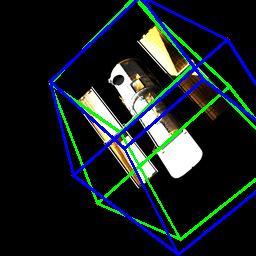
\includegraphics[width=\linewidth]{data/fig3.jpg} % First image
        \caption{Hubble Space Telescope, no background, 256x256 query image, $e_\mathrm{ADD}=2.925$, $e_{\mathrm{ADD}\text{-}\mathrm{S}}=1.183$ }
        \label{fig:fig3}
    \end{minipage}\hfill
    \begin{minipage}{0.45\linewidth}
        \centering
        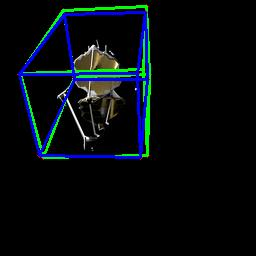
\includegraphics[width=\linewidth]{data/fig4.jpg} % Second image
        \caption{James Webb ST, no background, 256x256 query image, $e_\mathrm{ADD}=1.415$, $e_{\mathrm{ADD}\text{-}\mathrm{S}}=0.808$ }
        \label{fig:fig4}
    \end{minipage}
\end{figure}

\bigskip
\bigskip

\begin{figure}[h]
    \centering
    \begin{minipage}{0.45\linewidth}
        \centering
        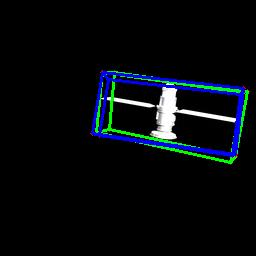
\includegraphics[width=\linewidth]{data/fig5.jpg} % First image
        \caption{Cosmos Link, no background, 256x256 query image, $e_\mathrm{ADD}=1.718$, $e_{\mathrm{ADD}\text{-}\mathrm{S}}=0.383$ }
        \label{fig:fig5}
    \end{minipage}\hfill
    \begin{minipage}{0.45\linewidth}
        \centering
        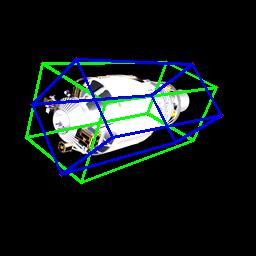
\includegraphics[width=\linewidth]{data/fig6.jpg} % Second image
        \caption{Rocket Body, no background, 256x256 query image, $e_\mathrm{ADD}=1.713$, $e_{\mathrm{ADD}\text{-}\mathrm{S}}=0.252$ }
        \label{fig:fig6}
    \end{minipage}
\end{figure}

\newpage

\begin{figure}[h]
    \centering
    \begin{minipage}{0.45\linewidth}
        \centering
        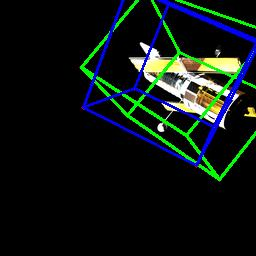
\includegraphics[width=\linewidth]{data/fig7.jpg} % First image
        \caption{Hubble Space Telescope, no background, 256x256 query image, $e_\mathrm{ADD}=6.514$, $e_{\mathrm{ADD}\text{-}\mathrm{S}}=1.571$ }
        \label{fig:fig7}
    \end{minipage}\hfill
    \begin{minipage}{0.45\linewidth}
        \centering
        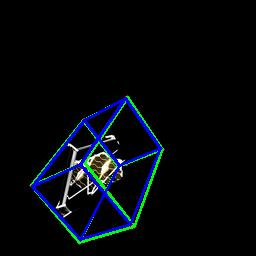
\includegraphics[width=\linewidth]{data/fig8.jpg} % Second image
        \caption{James Webb ST, no background, 256x256 query image, $e_\mathrm{ADD}=2.224$, $e_{\mathrm{ADD}\text{-}\mathrm{S}}=1.261$ }
        \label{fig:fig8}
    \end{minipage}
\end{figure}

\bigskip

\begin{figure}[h]
    \centering
    \begin{minipage}{0.45\linewidth}
        \centering
        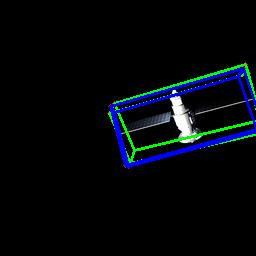
\includegraphics[width=\linewidth]{data/fig9.jpg} % First image
        \caption{Cosmos Link, no background, 256x256 query image, $e_\mathrm{ADD}=1.925$, $e_{\mathrm{ADD}\text{-}\mathrm{S}}=0.377$ }
        \label{fig:fig9}
    \end{minipage}\hfill
    \begin{minipage}{0.45\linewidth}
        \centering
        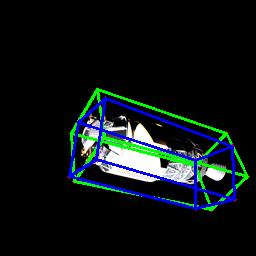
\includegraphics[width=\linewidth]{data/fig10.jpg} % Second image
        \caption{Rocket Body, no background, 256x256 query image, $e_\mathrm{ADD}=1.982$, $e_{\mathrm{ADD}\text{-}\mathrm{S}}=0.501$ }
        \label{fig:fig10}
    \end{minipage}
\end{figure}

\bigskip
\bigskip

From our observations, it's notable that the results are particularly less accurate with the Hubble Space Telescope. This seems to stem from errors in the ground truth poses, as pointed out by Haochen, another student working on the project, particularly an axis inversion. Also, we often notice that the estimations on the Rocket Body are rotated around the object's axis of symmetry compared to the ground truth pose. Thus, it is relevant to consider the $e_{\mathrm{ADD}\text{-}\mathrm{S}}$ metric in this case.

\bigskip

\cleardoublepage{}

While the above results are great, the issue is that in many instances, the estimation is rather inaccurate.
For completeness, we are now studying cases where Gen6D doesn't perform well, and we are trying to identify the reasons behind these shortcomings. The following text is provided by the authors to offer a clearer understanding of the intermediary results presented below: "[The column of vertical images] shows the viewpoint selection results. The first row shows the input image to the selector. The second row shows the input images rotated by the estimated in-plane rotation (left column) or the ground-truth in-plane rotation (right column) Subsequent 5 rows show the predicted (left) or ground-truth (right) 5 reference images with nearest viewpoints to the input image."

\bigskip
\bigskip

\begin{figure}[ht]
  \centering
  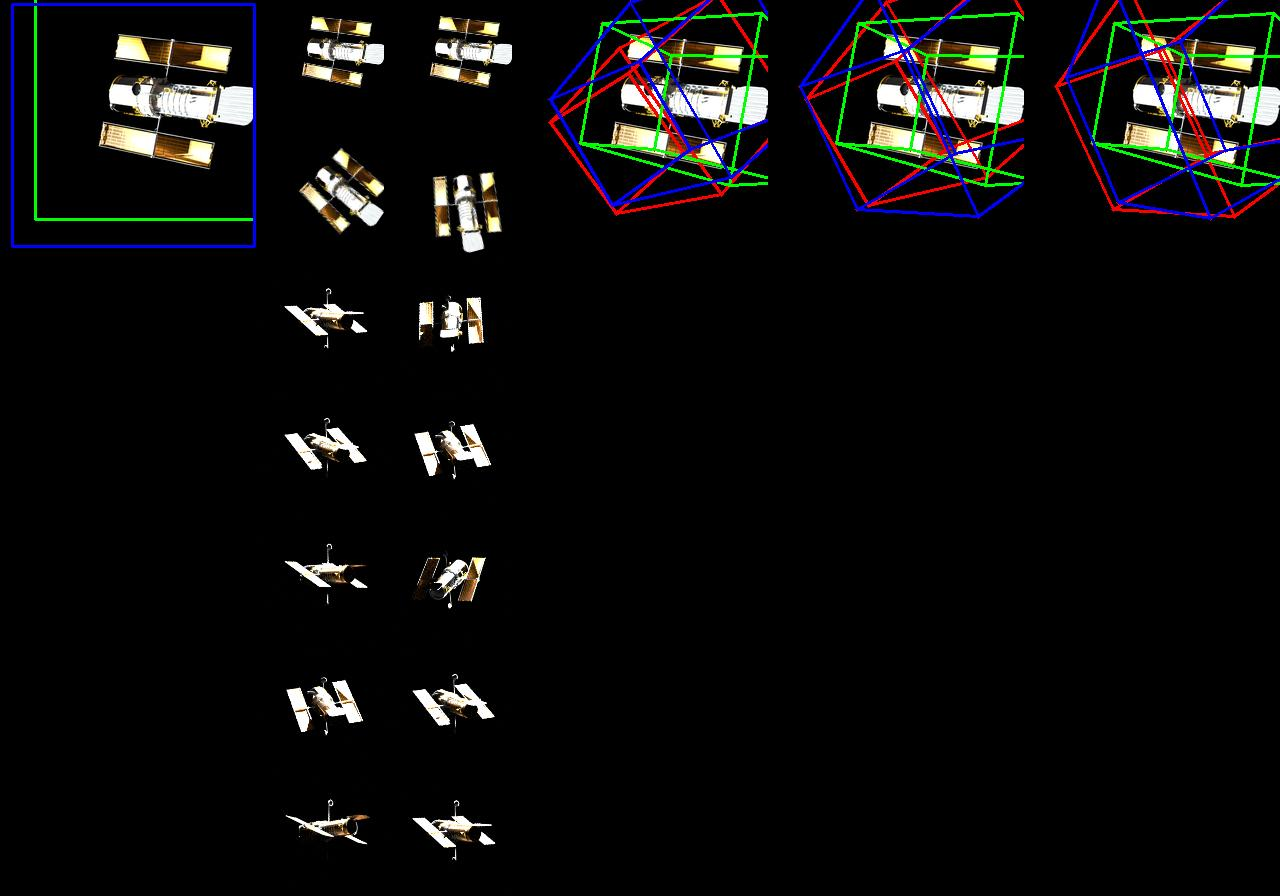
\includegraphics[width=\textwidth]{data/fig11.jpg}
  \caption{Hubble Space Telescope, no background, intermediary result of a poor estimation, $e_\mathrm{ADD}=9.577$, $e_{\mathrm{ADD}\text{-}\mathrm{S}}=5.196$}
  \label{fig:fig11}
\end{figure}

\bigskip

In Figure~\ref{fig:fig11}, we observe good detection of the object, however, the selection of the nearest viewpoint is lacking, ultimately leading to an inaccurate pose estimation. This supports the earlier explanations regarding errors in the ground truth poses for the Hubble Space Telescope. 

\bigskip
\cleardoublepage{}

\begin{figure}[ht]
  \centering
  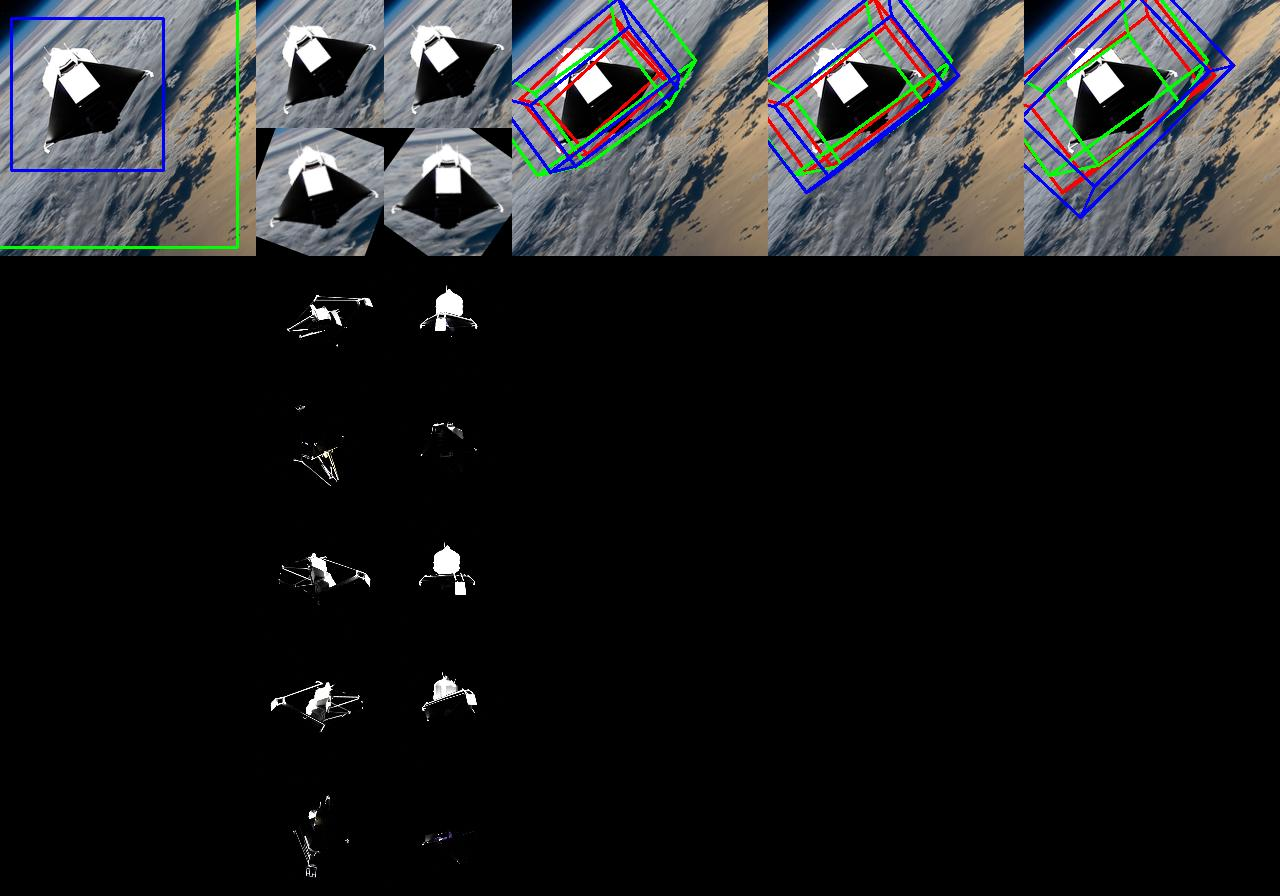
\includegraphics[width=0.8\textwidth]{data/fig12.jpg}
  \caption{James Webb Space Telescope, with earth rendered background, intermediary result of a poor estimation, $e_\mathrm{ADD}=10.934$, $e_{\mathrm{ADD}\text{-}\mathrm{S}}=4.317$}
  \label{fig:fig12}
\end{figure}

\bigskip

\begin{figure}[ht]
  \centering
  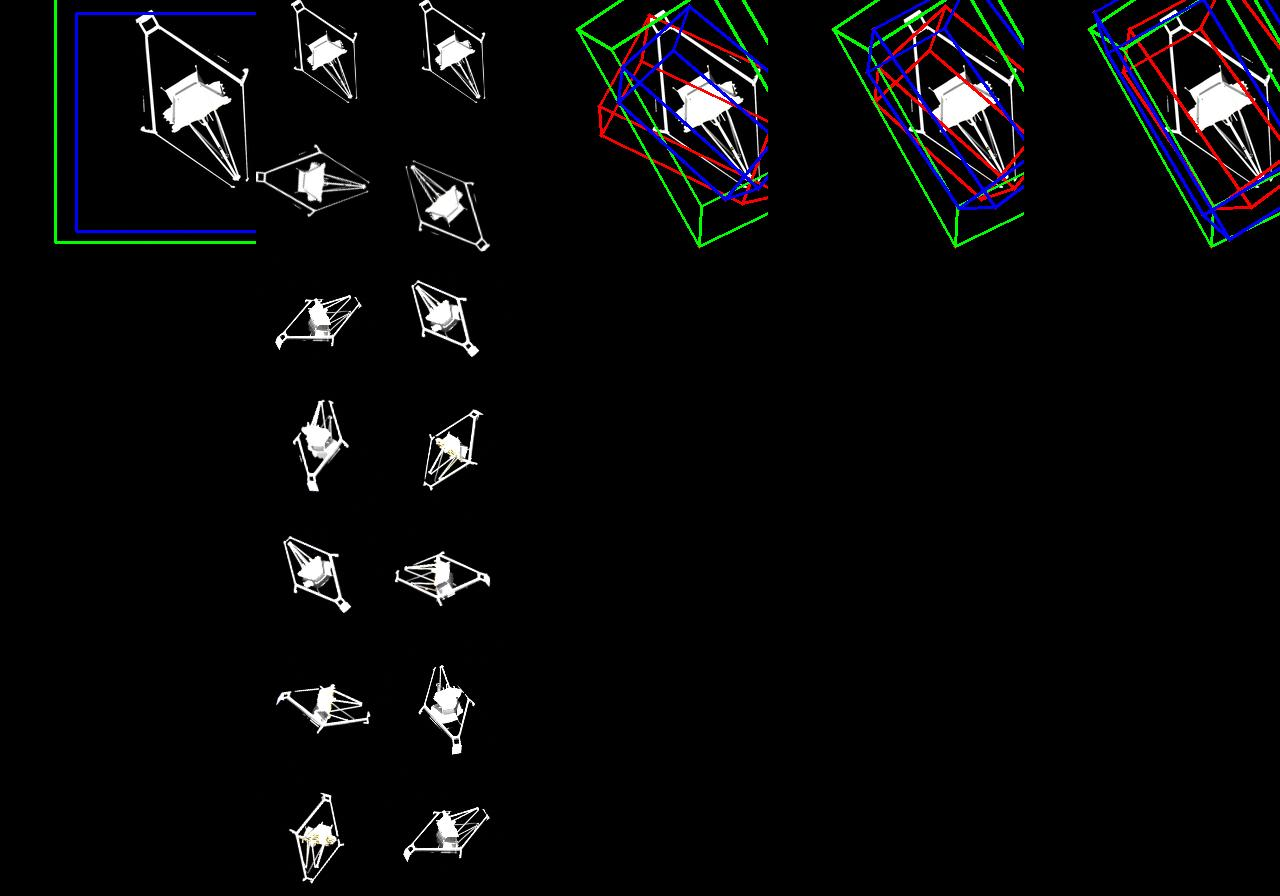
\includegraphics[width=0.8\textwidth]{data/fig16.jpg}
  \caption{James Webb Space Telescope, no background, intermediary result, $e_\mathrm{ADD}=1.060$, $e_{\mathrm{ADD}\text{-}\mathrm{S}}=0.556$}
  \label{fig:fig16}
\end{figure}

\bigskip

In Figure~\ref{fig:fig12}, we tested the model using reference images without a background and query images featuring the James Webb Telescope in front of the blue planet. While the object detection appears reasonably accurate, there is a significant difference in lighting conditions between the reference and query images. On the positive side, the refiner seems to work effectively as we observe an improvement in pose accuracy over the course of the three steps. Figure~\ref{fig:fig16} is another example of the refiner doing great.

\bigskip
\cleardoublepage{}

\begin{figure}[ht]
  \centering
  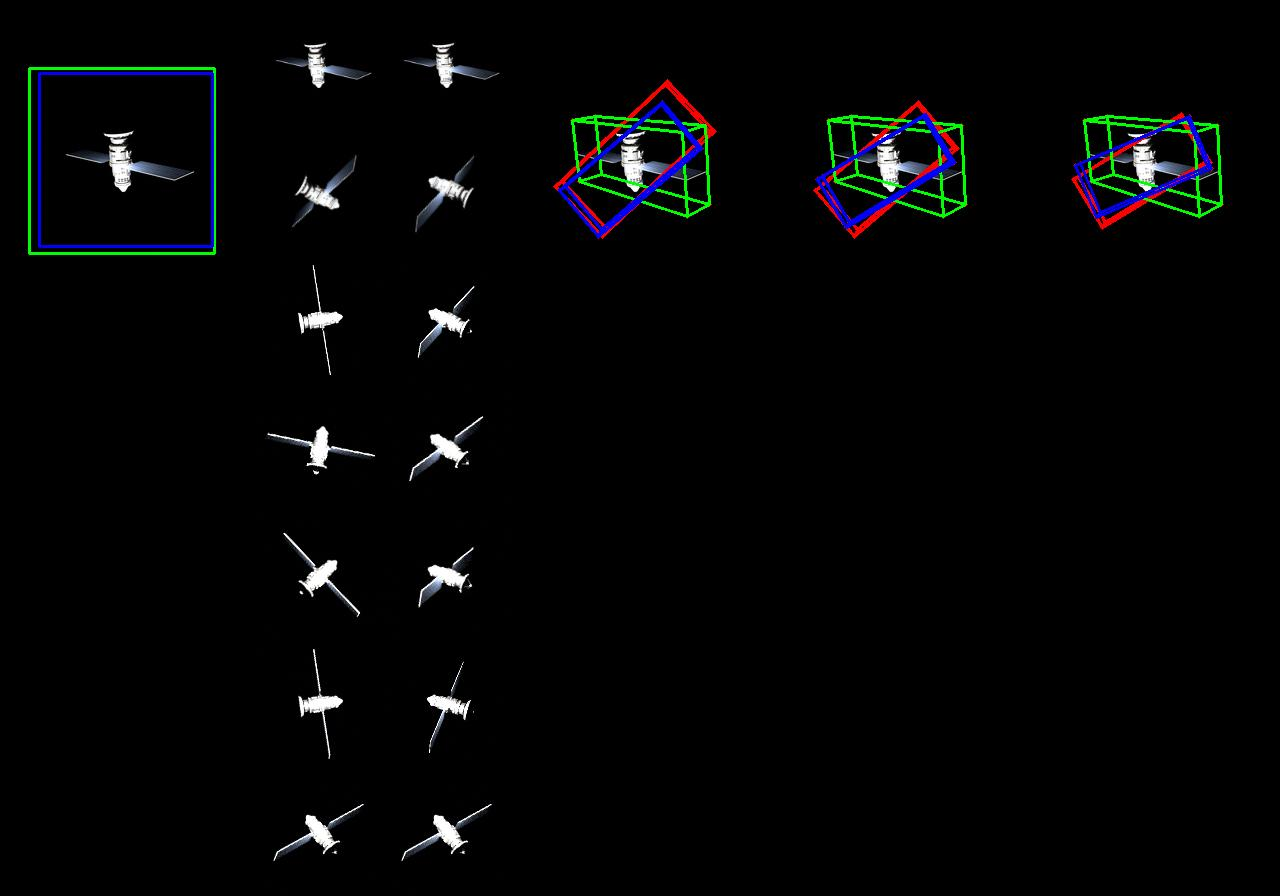
\includegraphics[width=\textwidth]{data/fig13.jpg}
  \caption{Cosmos Link, no background, intermediary result of a poor estimation, $e_\mathrm{ADD}=11.094$, $e_{\mathrm{ADD}\text{-}\mathrm{S}}=6.127$}
  \label{fig:fig13}
\end{figure}

\bigskip

In Figure~\ref{fig:fig13}, we have a perfect detection, reasonably favorable viewpoints and yet a poor estimated pose at the end. However, it appears that increasing the number of refinement steps could lead to an improvement.
\bigskip
\cleardoublepage{}

\begin{figure}[ht]
  \centering
  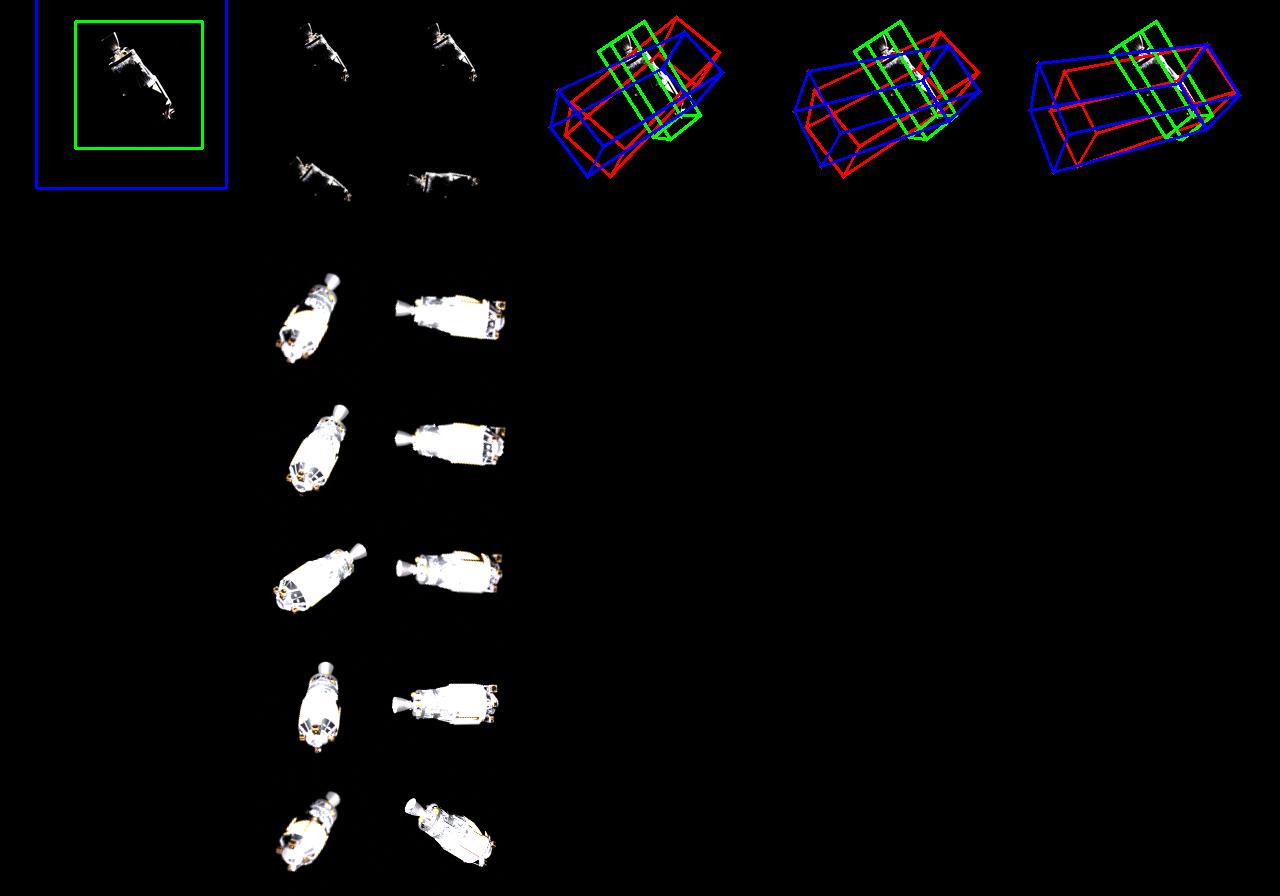
\includegraphics[width=0.8\textwidth]{data/fig14.jpg}
  \caption{Rocket Body, no background, intermediary result of a poor estimation, $e_\mathrm{ADD}=29.335$, $e_{\mathrm{ADD}\text{-}\mathrm{S}}=17.743$}
  \label{fig:fig14}
\end{figure}

\bigskip

\begin{figure}[ht]
  \centering
  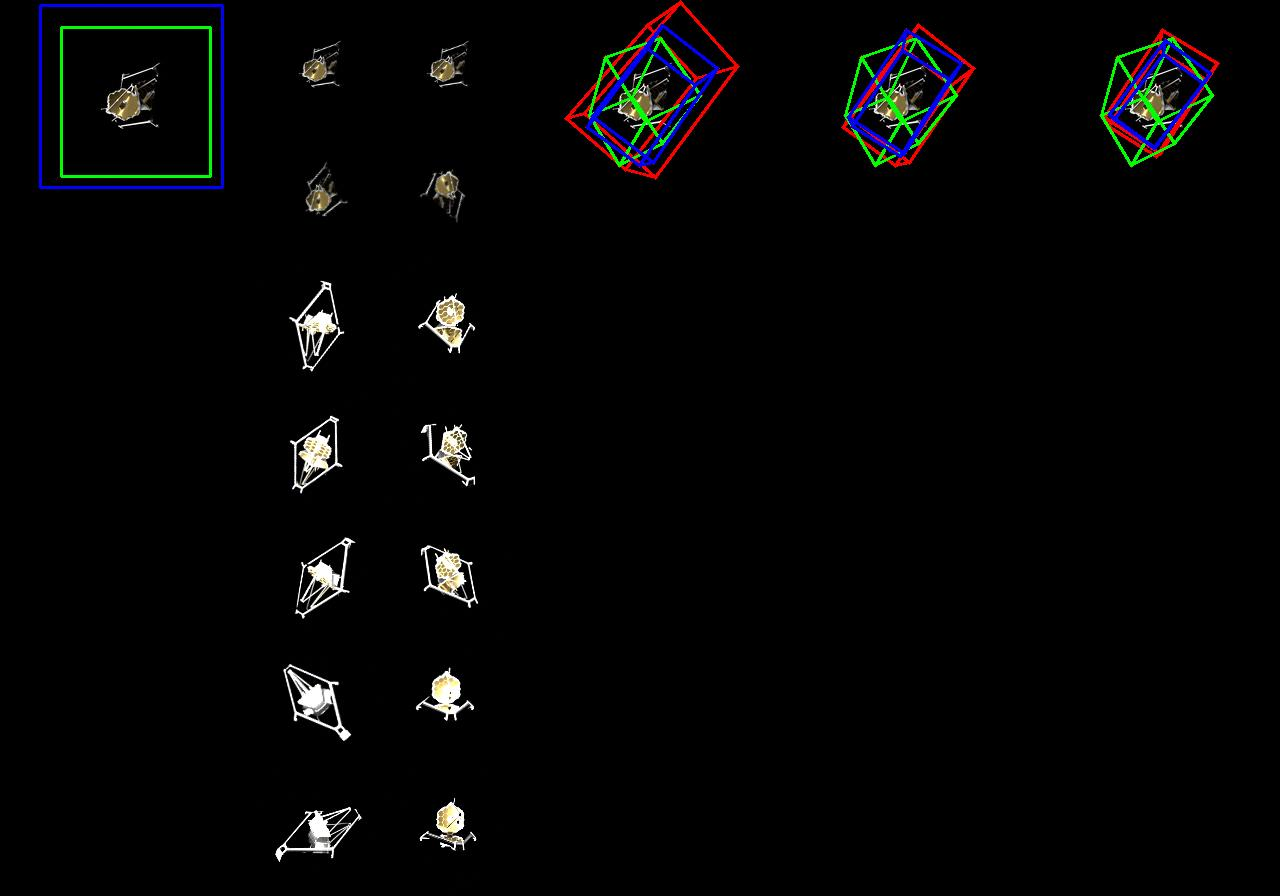
\includegraphics[width=0.8\textwidth]{data/fig15.jpg}
  \caption{James Webb Space Telescope, no background, intermediary result of a poor estimation, $e_\mathrm{ADD}=21.983$, $e_{\mathrm{ADD}\text{-}\mathrm{S}}=12.358$}
  \label{fig:fig15}
\end{figure}

\bigskip

In Figure~\ref{fig:fig14} and Figure~\ref{fig:fig15}, we are encountering large differences in terms of lighting conditions. Specifically, for the James Webb Space Telescope, the query image reveals the interior of the antenna, which is not present in any of the selected viewpoints. Therefore, we conclude that Gen6D struggles with accurately estimating poses when there are substantial variations in lighting conditions.



% !TeX root = ../main.tex
% Add the above to each chapter to make compiling the PDF easier in some editors.

\chapter{Ways of improvements}\label{chapter:ways_of_improvements}

As we observed in the previous chapter, Gen6D does not perform very well when generalizing to space objects. In this section, we will attempt to provide some tracks for improving the results of pose estimations.

\section{More diverse Reference Images}

Given the time constraints, we evaluated Gen6D under basic conditions, by using reference images from a folder of random synthetic images. To enhance the model's performance, one approach would be to diversify as much as possible the external conditions affecting the object's image through the camera, particularly lighting. As we observed, lighting plays a significant role during viewpoint selection. Having a more varied set of reference images would enable the model to better adapt to new conditions. Additionally, it's essential to ensure that the reference images are distributed as homogeneously as possible around the object. 

\section{Specialized Spacecraft Training Set}

To assess the ability of Gen6D to generalize, we opted not to retrain the model but instead utilized the pretrained model made available by the authors. This approach may introduce a challenge, as highlighted in Table~\ref{tab:tab}, where one of Gen6D's limitations is its training on everyday objects under favorable lighting conditions.

A viable solution would be to retrain Gen6D, focusing on specific components rather than the entire model. In particular, retraining only the detector and the viewpoint selector, while keeping the refiner as-is, could be effective. Indeed, retraining the detector would allow for the addition of new detecting scales for the object in query images, improving the accuracy of the estimated 2D bounding box. Additionally, retraining the viewpoint selector could prove beneficial for making pose estimations under poor lighting conditions. As for the refiner, as previously observed, it seems to perform pretty well and may not require retraining.

\section{Improve Object Detection and Viewpoint Selection Algorithms}
\fancyhead[C]{\small\textsc{5.3. Improve Object Detection and Viewpoint Selection Algorithms}}

A limitation of the current architecture of Gen6D is its detector: it requires predefined object scales in the query images for detection. This is a significant constraint, especially in competitive scenarios where the object could be very close or very far away. Additionally, the current necessity to resize query images leads to information loss and adds a manual step to the process.

To address this, the implementation of a \ac{FPN} could be a substantial improvement \cite{lin2017feature}. \ac{FPN}s are known for their efficiency in detecting objects at various scales through the utilization of a pyramidal hierarchy of deep convolutional networks. Incorporating a \ac{FPN} into Gen6D's architecture would enhance its ability to detect objects regardless of their distance or size in the query images, thus potentially improving overall performance.

During the detection and viewpoint selection phase, we could also think about relying more on the 3D model (for now it is only used to get the estimated 3D bounding box size) and the segmented images (currently unused), to get better results.

% !TeX root = ../main.tex
% Add the above to each chapter to make compiling the PDF easier in some editors.

\chapter{Conclusion}\label{chapter:conclusion}

In summary, after overcoming several software engineering challenges, we successfully reimplemented Gen6D for the \textsc{SpaceCraft} dataset. While the current results are somewhat disappointing, we have identified several promising tracks for future exploration to enhance the pose estimation accuracy.

\bigskip

Knowing that the dataset team has developed new renderings this semester with dozens of new models, there is ample opportunity to further test Gen6D. More importantly, this development opens up the potential for retraining the model. 

\bigskip

From a personal standpoint, this project was my first experience working as part of a significant and motivated team, and I thoroughly enjoyed the experience. It taught me to better organize my work, to operate on a remote server like Scitas Izar, to understand the functioning of a deep learning architecture in a practical, applied setting, to write Python scripts, and finally to improve my English skills through Zoom meetings and the writing of this very report.
% TODO: add more chapters here

\microtypesetup{protrusion=false}

\addchap{Abbreviations}
\begin{acronym}
	\itemsep-.25\baselineskip
	\acro{TUM}[TUM]{Technical University of Munich}
	\acro{EPFL}[EPFL]{École Polytechnique Fédérale de Lausanne}
	\acro{ESA}[ESA]{European Space Agency}
	\acro{DoF}[DoF]{Degrees of Freedom}
	\acro{CVLab}[CVLab]{Computer Vision Laboratory}
	\acro{SFM}[SFM]{Structure From Motion}
	\acro{ML}[ML]{Machine Learning}
	\acro{HPC}[HPC]{High Performance Computing}
	\acro{AI}[AI]{Artificial Intelligence}
	\acro{LEO}[LEO]{Low Earth Orbit}
	\acro{VGGNet}[VGGNet]{Visual Geometry Group Network}
	\acro{CNN}[CNN]{Convolutional Neural Network}
	\acro{DART}[DART]{Double Asteroid Redirection Test}
	\acro{ADD}[ADD]{Average Distance of Model Points}
	\acro{ADD-S}[ADD-S]{Average Closest Point Distance}
	% TODO: add acronyms
\end{acronym}

\cleardoublepage{}

%\listoffigures{}
%\listoftables{}

\appendix{}
\renewcommand{\thelstlisting}{A.\arabic{lstlisting}}
\setcounter{lstlisting}{0} % Reset the counter to start from 1
\chapter{Python Scripts}
\pagestyle{fancy}
\fancyhf{}
\fancyhead[C]{\small\textsc{A. Python Scripts}}

\begin{lstlisting}[style=pythonstyle, label=lst:1, caption=Python script \texttt{format.py} to randomly generate the training set and the test set based on a specified probability. Should be run from Gen6D's root folder.]
"""
Author:      Jeremy Chaverot
Date:        November 29, 2023
Description: Create the files val.txt, train.txt and test.txt according to a test percentage
"""

import os
import sys
import random


if __name__ == "__main__":

	# Check if the correct number of arguments is provided
    if len(sys.argv) != 3:
        print("Usage: python format.py <object_name> <test_percentage>")
        sys.exit(1)

    object = sys.argv[1]
    test_percentage = float(sys.argv[2])

    if (test_percentage < 0 or 1 < test_percentage):
        print("Wrong value for the variable <test_percentage>. Should be between 0 and 1 included.")
        sys.exit(1)

    # Get a list of all files in the folder
    all_files = os.listdir(f'data/SpaceCraft/{object}/images')

    # Filter the list to include only image files and exclude MacOS temporary files
    image_files = [file for file in all_files if file.lower().endswith(('.jpg')) and not file.startswith('._')]

    # Get the number of images in the folder
    num_images = len(image_files)

    # Iterate through each image and apply the transformation
    with open(f'data/SpaceCraft/{object}/train.txt', 'w') as train, open(f'data/SpaceCraft/{object}/test.txt', 'w') as test:
        for image_file in image_files:
            rand = random.random()
            image_path = 'SpaceCraft/hubble/images/' + image_file
            if (rand < test_percentage):
                test.write(image_path + '\n')
            else: train.write(image_path + '\n')

    print(f"Done splitting {num_images} images in train.txt and test.txt")
\end{lstlisting}

%\cleardoublepage{}
\bigskip

\begin{lstlisting}[style=pythonstyle, label=lst:2, caption=Python script \texttt{to\_jpg.py} to transform every images of a specified folder into \texttt{jpg} format.]
"""
Author:      Jeremy Chaverot
Date:        November 20, 2023
Description: Transform every images of a folder into jpg format.
"""

import os
import sys
from PIL import Image


def transform_image(image_path):
    img = Image.open(image_path)
    new_image_path = image_path.split('.')[0] + '.jpg'
    img.save(new_image_path)


if __name__ == "__main__":

	# Check if the correct number of arguments is provided
    if len(sys.argv) != 2:
        print("Usage: python to_jpg.py </path/to/your/images>")
        sys.exit(1)

    folder_path = sys.argv[1]

    # Get a list of all files in the folder
    all_files = os.listdir(folder_path)
    
    # Filter the list to include only image files and exclude MacOS temporary files
    image_files = [file for file in all_files if file.lower().endswith(('.png', '.jpg', '.jpeg', '.gif', '.bmp')) and not file.startswith('._')]
    
    # Get the number of images in the folder
    num_images = len(image_files)

    # Iterate through each image and apply the transformation
    for image_file in image_files:
        image_path = os.path.join(folder_path, image_file)
        transform_image(image_path)
        os.remove(image_path)

    print(f"Number of images transformed into .jpg: {num_images}")
\end{lstlisting}


%\cleardoublepage{}
\bigskip

\begin{lstlisting}[style=pythonstyle, label=lst:3, caption=Python script \texttt{quaternion\_to\_matrix.py} to transform a txt file with quaternions and the translation vector into multiple npy files containing the rotation matrix augmented with the translation vector.]
"""
Author:      Jeremy Chaverot
Date:        November 20, 2023
Description: Transform a txt file with quaternions and the translation vector into multiple npy files containing the rotation matrix augmented with the translation vector.
"""

import numpy as np
import sys
import os


def quaternion_to_matrix(Q, translation):
    """
        Covert a quaternion and translation into a full three-dimensional augmented rotation matrix.

        Input
        :param Q: A 4 element array representing the quaternion (qw, qx, qy, qz).
        :param translation: A 3 element array representing the translation (x, y, z).

        Output
        :return: A 3x4 element matrix representing the full 3D rotation matrix with
                 translation. This rotation matrix converts a point in the local
                 reference frame to a point in the global reference frame.
    """

    # Extract the values from Q
    qw = Q[0]
    qx = Q[1]
    qy = Q[2]
    qz = Q[3]

    # Extract the values from the translation vector
    x = translation[0]
    y = translation[1]
    z = translation[2]

    # First row of the rotation matrix
    r00 = 2 * (qw * qw + qx * qx) - 1
    r01 = 2 * (qx * qy - qw * qz)
    r02 = 2 * (qx * qz + qw * qy)

    # Second row of the rotation matrix
    r10 = 2 * (qx * qy + qw * qz)
    r11 = 2 * (qw * qw + qy * qy) - 1
    r12 = 2 * (qy * qz - qw * qx)

    # Third row of the rotation matrix
    r20 = 2 * (qx * qz - qw * qy)
    r21 = 2 * (qy * qz + qw * qx)
    r22 = 2 * (qw * qw + qz * qz) - 1

    # 3x3 rotation matrix
    rot_matrix_augm = np.array([[r00, r01, r02, x],
                                [r10, r11, r12, y],
                                [r20, r21, r22, z]])

    return rot_matrix_augm


if __name__ == "__main__":

    # Check if the correct number of arguments is provided
    if len(sys.argv) != 3:
        print("Usage: python quaternion_to_matrix.py </path/to/your/text/file> </path/to/the/pose/folder>")
        sys.exit(1)

    file_path = sys.argv[1]
    pose_folder_path = sys.argv[2]
    file_content = None

    try:
        with open(file_path, 'r') as file:
            file_content = file.read()
    except FileNotFoundError:
        print(f"The file {file_path} was not found.")
        sys.exit(1)
    except Exception as e:
        print(f"An error occurred: {e}")
        sys.exit(1)

    poses = file_content.split('\n')[:-1]
    
    # Iterate through each pose and apply the transformation
    for pose in poses:
        image_id, obj_id, qw, qx, qy, qz, x, y, z = pose.split(',')
        Q = np.array([qw, qx, qy, qz], dtype=np.float32)
        translation = np.array([x, y, z], dtype=np.float32)
        matrix = quaternion_to_matrix(Q, translation)
        np.save(pose_folder_path + '/pose' + str(int(image_id)), matrix)

    print(f"Number of transformation processed: {len(poses)}")
\end{lstlisting}

%\cleardoublepage{}
\bigskip

\begin{lstlisting}[style=pythonstyle, label=lst:4, caption=Python script \texttt{invert\_mask.py} to invert the masks from a specified folder. We aim to have a black object set against a white background.]
"""
Author:      Jeremy Chaverot
Date:        December 10, 2023
Description: Invert the masks from a given folder.
"""

import cv2
import os
import sys


def inverse_masks_in_folder(folder_path):
	# Iterate through the list of files at the specified path
    for filename in os.listdir(folder_path):
    	# Filter to include only png image files and exclude MacOS temporary files
        if filename.endswith(".png") and not filename.startswith('._'):
            mask_path = os.path.join(folder_path, filename)
            try:
                # Read the mask image
                mask = cv2.imread(mask_path, cv2.IMREAD_GRAYSCALE)
                if mask is None:
                    print(f"Failed to read image: {mask_path}")
                    continue

                # Invert the mask
                inverted_mask = cv2.bitwise_not(mask)

                # Save the inverted mask with a temporary name
                temp_path = os.path.join(folder_path, "temp_" + filename)
                cv2.imwrite(temp_path, inverted_mask)

                # Delete the original mask
                os.remove(mask_path)

                # Rename the inverted mask to the original filename
                os.rename(temp_path, mask_path)
                print(f"Inverted and replaced mask for: {mask_path}")
            except Exception as e:
                print(f"Error processing {mask_path}: {e}")


if __name__ == "__main__":

	# Check if the correct number of arguments is provided
    if len(sys.argv) != 2:
        print("Usage: python invert_mask.py <folder_path>")
        sys.exit(1)

    folder_path = sys.argv[1]
    inverse_masks_in_folder(folder_path)
\end{lstlisting}

%\cleardoublepage{}
\bigskip

\begin{lstlisting}[style=pythonstyle, label=lst:5, caption=Python script \texttt{resize.py} designed to alter an image's size with respect to a specified resize factor.]
"""
Author:      Jeremy Chaverot
Date:        January 01, 2024
Description: Resize the images from a given folder.
"""

import os
import sys
from PIL import Image


def resize_images(folder_path, resize_factor):
	# Iterate through the list of files at the specified path
    for filename in os.listdir(folder_path):
    	# Filter to include only png image files and exclude MacOS temporary files
        if filename.endswith(".png") and not filename.startswith('._'):
            img_path = os.path.join(folder_path, filename)
            with Image.open(img_path) as img:
                # Calculate new size
                new_size = tuple([int(dim / resize_factor) for dim in img.size])
                # Resize the image
                resized_img = img.resize(new_size, Image.ANTIALIAS)
                # Save the resized image with a different name temporarily
                temp_path = os.path.join(folder_path, "temp_" + filename)
                resized_img.save(temp_path)

            # Delete the original image
            os.remove(img_path)

            # Rename the resized image to the original filename
            os.rename(temp_path, img_path)


if __name__ == "__main__":

	# Check if the correct number of arguments is provided
    if len(sys.argv) != 3:
        print("Usage: resize.py <folder_path> <resize_factor>")
        sys.exit(1)

    folder_path = sys.argv[1]
    factor = int(sys.argv[2])

    resize_images(folder_path, factor)
\end{lstlisting}

%\cleardoublepage{}

%\begin{lstlisting}[language=Python, label=lst:6, caption=Python script \texttt{.py}.]

%\end{lstlisting}

\cleardoublepage{}

\chapter{Scitas Izar Setup Tutorial}
\fancyhead[C]{\small\textsc{B. Scitas Izar Setup Tutorial}}

\begin{lstlisting}[style=bashstyle, caption={Bash script \texttt{execute.sh} to run a machine learning model on Scitas Izar EPFL. While the overall structure remains consistent, this script is specific to Gen6D's architecture, further discussed later.}]
#!/bin/bash
#SBATCH --chdir /scratch/izar/jchavero
#SBATCH --partition=gpu
#SBATCH --qos=gpu_free
#SBATCH --gres=gpu:2
#SBATCH --nodes=1
#SBATCH --ntasks-per-node=1
#SBATCH --cpus-per-task=1
#SBATCH --mem 16G

echo STARTING AT `date`

echo "Loading modules"
module load gcc openmpi py-torch py-torchvision cuda

echo "Launching the virtual environment"
source ~/opt/izar1/venv-gcc/bin/activate

echo "Navigating to the directory and executing the task"
cd ~/Gen6D                                    
python eval.py --cfg configs/gen6d_pretrain.yaml --object_name spacecraft/hubble

echo FINISHED AT `date`
\end{lstlisting}

\noindent Then to run the script we use the following command:
\begin{lstlisting}[style=bashstyle, caption=Linux command to run the bash script.]
	$ sbatch execute.sh
\end{lstlisting}





\cleardoublepage{}
\microtypesetup{protrusion=true}

\printbibliography{}
\end{document}
